% ============================================================================
% 第 7 章  迈向同调镜像对称  （原书 pp.110–127，PDF pp.113–130）
% ============================================================================
\section{迈向同调镜像对称}\label{ch:07}

% 原书公式在全书范围内连续编号：本章自 (101) 起、至 (120) 止，共 20 个编号公式。
% main.tex 已采用全局连续编号；此处补设计数器为 100，保证本章首个编号公式
% 恰为 (101)。若前几章的公式计数已经连续到 100，则本行只是空操作。
\setcounter{equation}{100}

\takeaway{%
  核心图像：弦论用一维的弦取代零维点粒子；镜像对称让一对 Calabi–Yau 流形上的 A-模型与 B-模型互换。\\
  数学工具：Kähler 几何与 Hodge 理论、Calabi–Yau 流形、层与导出范畴、Floer 上同调与 $A_\infty$-范畴。\\
  主要结论：镜像对称猜想（猜想~\ref{con:7.8}）与同调镜像对称猜想（猜想~\ref{con:7.26}）；SYZ 猜想用特殊拉格朗日环面的对偶纤维化构造镜像对。%
}

\subsection{镜像对称的物理起源}\label{sec:7.1}

镜像对称是弦论中涌现的一种现象。弦论是高能理论物理的一个分支，试图把引力与标准粒子物理统一起来，并力图使自己成为涵盖量子引力的“万物理论”（\cite{BBS07}）。在弦论之前，物理学历来依赖经典几何；而大约发端于 20 世纪 60 年代末、70 年代初的弦论，则建立在一种更丰富的几何之上——量子几何——同时也积极促成了后者的建立。量子几何的新特征只在 Planck 尺度 $\hbar\sim10^{-35}$ m 才显现（更广泛的讨论见 \cite{Gre97}）。
% [Tutor Note: 【勘误】原文把 Planck 尺度写成“ℏ ∼ 10^{-35} m”。ℏ 的量纲是作用量，10^{-35} m 实际上是 Planck 长度 l_P = (ℏG/c^3)^{1/2}；作者以此代指普朗克尺度，译文照印。]

量子几何的核心想法，是把粒子当作零维点状客体的量子场论描述，替换为弦的描述。弦是非常小的一维客体，或为闭圈，或为开线段；其不同的振动模式决定质量、电荷与自旋等基本性质，从而有效复制了所有基本粒子与力的载体的特征和相互作用方式（\cite{BBS07}）。

然而，要使这个模型在物理与数学上都自洽，就必须为弦所栖居的环境时空增添额外的维度，好让弦沿这些维度振动。于是，Minkowski 时空 $\mathbb R^4$ 必须换成某个更高维的流形 $M=\mathbb R^4\times X$。弦论的后续版本成功融入了超对称的概念——它在玻色子与费米子之间建立一种物理对偶——并由此催生了五种主要的超弦理论（参见 \cite{Zwi09}），它们都要求 $X$ 是某个特定的六维紧 Riemann 流形。
% [Tutor Note: 【背景】五种超弦理论即 I 型、IIA 型、IIB 型、SO(32) 杂化与 E_8×E_8 杂化。超弦的临界维数是 10：四维 Minkowski 时空加上六维紧化的内部流形 X，故 X 是复三维的。]

为了与我们四维 Minkowski 极限下的实验相符，六个额外的（空间）维度在宏观上必须不可探测，也就是说，它们必须在 $\operatorname{diam}(X)\sim\hbar$ 的尺度内“卷”回自身。这样的模型称为紧化。若把超对称计入，$X$ 就必须取某个三维复 Calabi–Yau 流形或簇（见 \cite{GHJ03} 与 \cite{YN10}；下一节将引入这种对象）。弦在这些维度里扫出紧的二维曲面，称为世界面（与之相对，点粒子扫出的是世界线）；物理学家在世界面上构造二维超共形量子场论（SCFT），其性质取决于 $X$ 的不变量（\cite{GHJ03}）。

20 世纪 80 年代末，人们发现各种超弦理论之间存在若干非平凡的物理对偶，其中最突出的是连接 IIA 型与 IIB 型弦理论的 T-对偶；它蕴含两者的 SCFT 等价，从而所描述的物理也等价（参看 \cite{BBS07}）。人们又发现，这种等价反映在各自底层 Calabi–Yau 流形的某些不变量之间的对应上，于是称这样一对流形构成“镜像对”。随后的研究很快自成气候，使镜像对称成为一门名副其实的数学分支（\cite{ABCp09}）。计数几何是研究几何问题之解的计数的领域，它从这一新成员中获益良多（\cite{HKKp03} 有讨论）：例如，可以嵌入五次 Calabi–Yau 流形（如本章末图~\ref{fig:15} 所画的那个）的直线数目是 2875，而圆锥曲线的数目是 609250（见 \cite{YN10}）。
% [Tutor Note: 【勘误】原文称五次 Calabi–Yau 流形的图像见“本章末的 Figure 15”。但原书 Figure 15（p.127）是 SYZ 猜想的示意图，并非五次流形的图像；此处疑为作者交叉引用笔误，译文照印。]

到 80 年代末，许多由来已久的这类谜题已被解开。1991 年，物理学家 Candelas、de la Ossa、Green 与 Parkes 的研究 \cite{CdGP91} 重新点燃了人们对这一题目的兴趣：他们证明，镜像对称可以把模型 Calabi–Yau 流形 $X$ 上的困难问题化为其镜像流形 $X^\dagger$ 上容易得多的问题，例如预言嵌入有理曲线的数目，且维数不限！
% [Tutor Note: 【含糊】原文作“rational curves of any dimension”（任意维数的有理曲线）。曲线总是一维的，此处疑指“任意次数（degree）”的有理曲线计数，即 [CdGP91] 预言的 Gromov–Witten 不变量；译文照印原文措辞。]

目前，关于镜像对称最重要、形式化也最好的陈述之一是猜想~\ref{con:7.8}（参看 \cite{Aur09}），它把一对 $(X,X^\dagger)$ 以下述方式联系起来：

\begin{quote}
$X$ 上的 A-模型对应于 $X^\dagger$ 上的 B-模型，而 $X$ 上的 B-模型对应于 $X^\dagger$ 上的 A-模型。
\end{quote}

粗略地说，（拓扑扭化的非线性 sigma）A-模型只挑选流形的辛结构，而（拓扑扭化的非线性 sigma）B-模型只捕捉其复的、代数几何的特征；人们常说 A-侧与 B-侧（这一术语来自前述的 IIA 型与 IIB 型超弦理论）。理解这个猜想是第~\ref{sec:7.2} 节的目标。
% [Tutor Note: 【背景】A-模型是拓扑扭化的 IIA 型非线性 sigma 模型，只依赖辛结构（有 B-场时依赖复化 Kähler 类）；B-模型是拓扑扭化的 IIB 型模型，只依赖复结构。扭化（twisting）指把世界面上的超共形代数改造成拓扑场论所需的 BRST 算子。]

到 20 世纪 90 年代初，大部分数学机器都建立在“闭”弦理论之上：其对象是闭弦，它们形成极小的圈，扫出管状世界面。然而，一旦考虑端点落在 D-膜上的开弦，新的研究动力便出现了。$p$-膜是 $p$ 维的广义弦，扫出一个 $(p+1)$ 维时空体积（\cite{Moo05}）。D-膜是其中一类特殊对象：它给端点落在其上的开弦世界面加上 Dirichlet 边界条件（“D”即由此而来）。图~\ref{fig:14} 画出了一些可能的构型。

\begin{figure}[htbp]
  \centering
  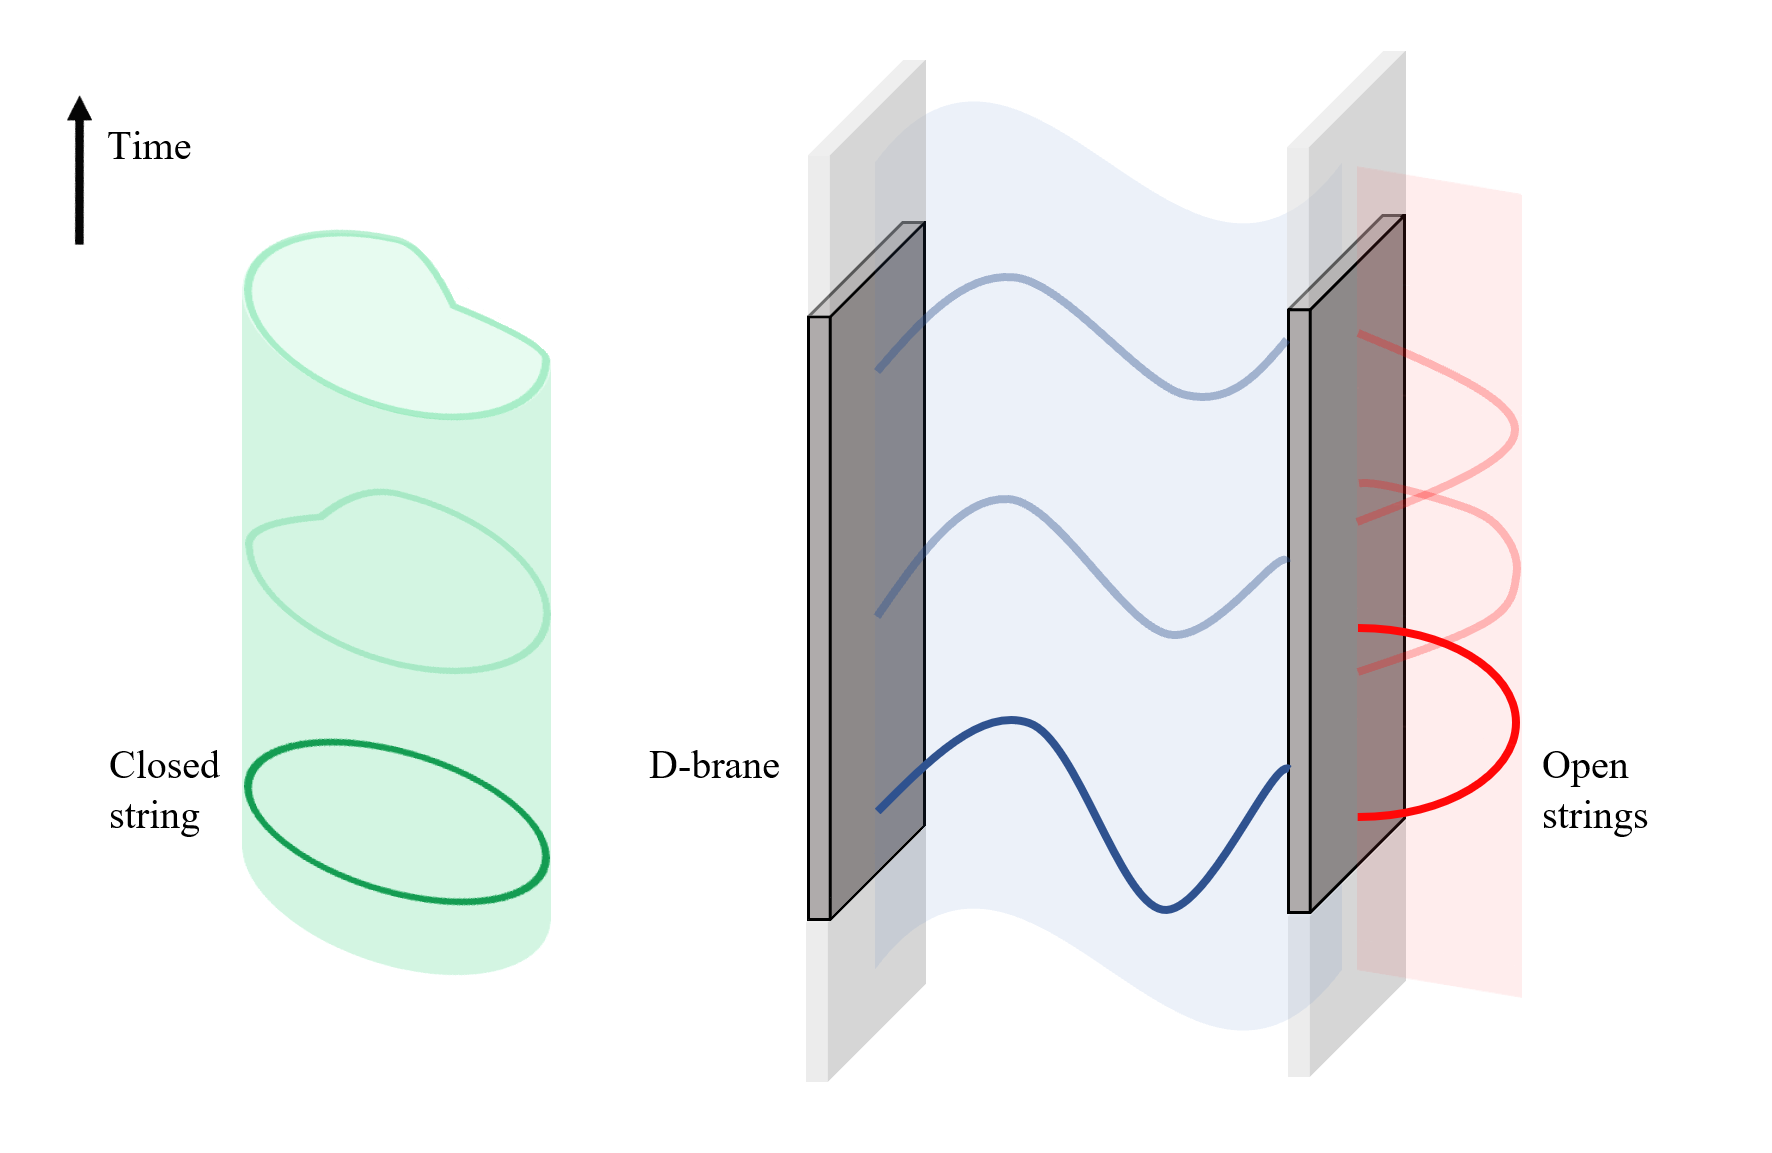
\includegraphics[width=0.55\linewidth]{fig14.png}
  \caption{一些可能的弦构型及其世界面。蓝色开弦的边界落在不同的 D-膜上，这应会令人想起第 5 章反复讨论的某个问题……\hfill（原书 p.111）}
  \label{fig:14}
\end{figure}

量子场论的公理早已提示，D-膜应当被组织成数学范畴（参看 \cite{ABCp09}）。具体说来，在 A-模型中相关对象（A-膜）是带平坦线丛的拉格朗日子流形，而在 B-模型中则是带有全纯向量丛的复子流形（B-膜）。第~\ref{sec:7.3} 节将考察这两种类型。
% [Tutor Note: 【背景】“A-膜是带平坦线丛的拉格朗日子流形”只是底线情形；一旦引入 B-场，平坦线丛须换成曲率为 iB|_L 的酉联络（见注 7.24），更一般地还要用扭复形与分级拉格朗日子流形来描述。]

1994 年，受开弦观点的推动，数学家 M. Kontsevich 登场。在苏黎世举行的国际数学家大会（ICM）上，他给出了镜像对称猜想的同调精细化（发表于 \cite{Kon94}）。他断言：给定满足 $c_1(X)=0$ 的 $2n$ 维辛流形 $(X,\omega)$ 与对偶的 $n$ 维复代数流形 $X^\dagger$，

\begin{quote}
“由 Fukaya 范畴 $\mathcal F(X)$（或某个适当扩大后的范畴）构造的导出范畴，等价于 $X^\dagger$ 上凝聚层的导出范畴”，
\end{quote}

从而在开弦理论与三角范畴之间画出一条平行线。这个论证有一半我们已经熟悉。于是，第~\ref{sec:7.3} 节的目标是尽可能合理地解释镜像那一侧究竟是什么，以及它如何嵌入猜想~\ref{con:7.26}——那是 Kontsevich 断言的一个（过于宽泛的）版本（\cite{Fuk02a} 中有概述）。最后我们还会提到 Strominger、Yau 与 Zaslow 三人的一个猜想：他们 1996 年的工作 \cite{SYZ96} 定性地说明了如何“具体地”构造一对镜像 Calabi–Yau 流形。
% [Tutor Note: 【含糊】Kontsevich 所说的“适当扩大后的范畴”，在本书语境中即对 $\mathcal F(X)$ 取分裂封闭扭复形所得的导出范畴 $\mathsf D^\pi(\mathcal F(X))$（也可换成 wrapped 版本），使得 Hom 集恰为 Floer 上同调；详见第 3.5、3.6 节与 \cite{Fuk02a} 第 2 章。]

在继续之前，我们要强调：弦论及其各分支（包括镜像对称）的严格数学表述，至今仍远未完成，这也是它们带有猜想性质的原因。除此之外，我们还选择一条更直接、更不分散的进路，把所有必要的要素只讨论到定义层面。除了常识之外，这样做还有两方面理由：一方面，我们希望给出一个自足的综述，使我们看清迄今发展出的理论嵌入“更大图景”的何处；另一方面，本章也充当一张试探性的路线图，为可能的后续工作指明方向。

\subsection{镜像对称}\label{sec:7.2}

镜像对称猜想的主角是 Calabi–Yau 流形。我们要给出的定义需要先在 Kähler 几何的领域里做几步准备。首先，我们绕开全纯图册，给出复流形的另一种刻画（证明在文献中很容易找到）。

\begin{Lem}[Newlander--Nirenberg 定理]\label{lem:7.1}
设 $M^n=(M,J)$ 是 $\mathbb C$ 上 $n$ 维近复流形。则它是复流形（如第 5.1 节所述），当且仅当其近复结构 $J\in\mathcal T^{1,1}(M)$ 使 Nijenhuis 张量
\[
N_J(X,Y):=[X,Y]+J\bigl([JX,Y]+[X,JY]\bigr)-[JX,JY]
\]
对所有 $X,Y\in\mathfrak X(M)$ 为零（此时称 $J$ 为 $M$ 的\textbf{可积复结构}）。
\end{Lem}

它与复流形通常定义的相容性，源于 Nijenhuis 张量 $N_J$ 正是（$J$-）全纯函数存在的障碍：所谓全纯函数，就是光滑函数 $f\in C^\infty(M,\mathbb C)$，满足 $(df)_x\circ J=i(df)_x$ 对一切 $x\in M$ 成立（其中 $df:=d(\operatorname{Re}(f))+i\,d(\operatorname{Im}(f))$；可与 $J$-全纯曲线的定义 5.7 对照）。
% [Tutor Note: 【易错】Newlander–Nirenberg 定理常被简写为“Nijenhuis 张量为零即复结构可积”。要点在于 J 必须属于 C^1 且 N_J 是 TM 值 2-形式，等式 N_J(X,Y)=0 的符号约定随 [JX,JY] 项的系数而异；本书采用 N_J = [X,Y] + J([JX,Y]+[X,JY]) − [JX,JY]。]

由于固定某个 Riemann 度量（它总是存在）之后，辛流形自然成为近复流形，我们有时用记号 $(M^{2n},J,\omega)$ 来强调它还带有复结构，其中维数 $2n$ 是就 $\mathbb R$ 而言的。

\begin{Rem}\label{rem:7.2}
下面是复微分几何的一些基本概念（更易消化的介绍见 \cite{Sil12} 第 14、15 章）。
\begin{itemize}
  \item $M^{2n}$ 上的近复结构 $J\in\mathcal T^{1,1}(M)\cong\Gamma(\operatorname{End}(TM))$ 可以延拓到复化切丛 $TM^{\mathbb C}:=TM\otimes\mathbb C$（其纤维为 $T_xM^{\mathbb C}=T_xM\otimes\mathbb C$）：只需令 $J(X\otimes z):=J(X)\otimes z$ 对一切 $X\in\mathfrak X(M)$、$z\in\mathbb C$ 成立。这样得到特征值为 $\pm i$ 的张量场 $J\in\mathcal T^{1,1}(TM^{\mathbb C})$（按定义如此），于是可把 $TM^{\mathbb C}$ 分解为两个特征子丛，即 $TM^{\mathbb C}=TM^{1,0}\oplus TM^{0,1}$。同样可构造复化余切丛 $T^*M^{\mathbb C}:=T^*M\otimes\mathbb C=T^*M^{1,0}\oplus T^*M^{0,1}$。
  \item 特别地，谈论 $(M,J)$ 上的复值形式才有意义：令 $\Lambda^{p,q}(T^*M^{\mathbb C}):=\Lambda^p(T^*M^{1,0})\wedge\Lambda^q(T^*M^{0,1})$，则\textbf{$(p,q)$-形式}是 $\Omega^{p,q}(M):=\Gamma(\Lambda^{p,q}(T^*M^{\mathbb C}))$ 的元素。然后定义
  \[
  \Omega^r(M):=\bigoplus_{p+q=r}\Omega^{p,q}(M)\;.
  \]
  若假定 $M$ 是复流形，则可把 $\Omega^{1,1}(M)$ 看成由 $dz\wedge d\bar z$ 局部张成的空间，其中 $z=x+iy\in C^\infty(M,\mathbb C)$ 是某个（全纯）坐标函数（从而 $dz\circ J=i\,dz=i\,dx-dy$）。
  \item 设 $\pi^{p,q}:\Lambda^r(T^*M^{\mathbb C}):=\bigoplus_{p+q=r}\Lambda^{p,q}(T^*M^{\mathbb C})\to\Lambda^{p,q}(T^*M^{\mathbb C})$ 表示到第 $(p,q)$ 个直和项的投影。于是（延拓后的）外微分算子 $d:\Omega^\bullet(M)\to\Omega^{\bullet+1}(M)$ 给出两个微分
  \[
  \partial_p:=\pi^{p+1,q}\circ d:\Omega^{p,q}(M)\to\Omega^{p+1,q}(M)\;,\qquad
  \bar\partial_q:=\pi^{p,q+1}\circ d:\Omega^{p,q}(M)\to\Omega^{p,q+1}(M)\;.
  \]
  对函数 $f\in C^\infty(M,\mathbb C)$，有 $d^0f=\partial^0f+\bar\partial^0f$，因此特别地，$f$ 全纯当且仅当 $\bar\partial^0f=0$。
  \item 事实上，在复流形 $M$ 上，对任意形式 $\nu\in\Omega^r(M)$ 都有 $d=\partial+\bar\partial$；又由 $0=d^2\nu=\partial^2\nu+(\partial\bar\partial+\bar\partial\partial)\nu+\bar\partial^2\nu$ 可推出：$\partial,\bar\partial$ 分别是上链复形 $\Omega^{\bullet,q}$ 与 $\Omega^{p,\bullet}$ 的（反交换的）上边缘算子。于是，对一切 $p,q\in\mathbb Z$，Dolbeault 上同调群
  \begin{equation}\label{eq:7.101}
  H^{p,q}_{Db}(M):=\frac{\ker(\bar\partial_q)}{\operatorname{im}(\bar\partial_{q-1})}
  \end{equation}
  都有良好定义。
  \item 进而，Dolbeault 定理给出同构
  \begin{equation}\label{eq:7.102}
  H^{p,q}_{Db}(M)\cong H^q(M;\Omega^{p,0}_M)\;,
  \end{equation}
  其中右端是与 $M$ 上 $(p,0)$-形式层 $\Omega^{p,0}_M$ 相伴的第 $q$ 个层上同调群（层上同调可参阅 \cite{Har77} 第 III 章）。这个结果可以看作 de Rham 定理的复类比。
\end{itemize}
\end{Rem}
% [Tutor Note: 【易错】第 (101) 式中 $\ker$ 与 $\operatorname{im}$ 都是无穷维空间，逐点定义的商只在复流形上才有意义；但当 $M$ 紧 Kähler 时，Hodge 定理保证 $H^{p,q}_{Db}(M)$ 有限维。另注意原书公式编号自 (101) 起，是全书连续编号，非按章重新计数。]
% [Tutor Note: 【含糊】第二条把 $\Lambda^{p,q}$ 写成 $\Lambda^p(T^*M^{1,0})\wedge\Lambda^q(T^*M^{0,1})$，严格说应是张量积 $\otimes$（两个向量丛一般不能作外积）；这是文献中常见的不严格写法，译文照印。]

\begin{Def}\label{def:7.3}
设 $M^n=(M,J)$ 是复流形，并配有 Riemann 度量 $h\in\Gamma(T^*M\otimes T^*M)$。若 $h(X,Y)=h(JX,JY)$ 对一切 $X,Y\in\mathfrak X(M)$ 成立（这意味着 $TM$ 上有一个光滑变化的正定 Hermitian 内积），则称 $h$ 为 \textbf{Hermitian 度量}，并称 $(M,J,h)$ 为 \textbf{Hermitian 流形}。注意这些数据确定了一个实 $(1,1)$-形式 $\kappa:=-\operatorname{Im}(h)\in\Omega^2(M)$，它满足 $\kappa(J\cdot,\cdot)=h(\cdot,\cdot)$。

此外，若还满足 $\nabla J=0$（其中 $\nabla$ 是 $h$ 的 Levi–Civita 联络），等价地若 $d\kappa=0$ 或 $\nabla\kappa=0$，则 $h$ 还是 \textbf{Kähler 度量}。此时称 $M=(M,J,h,\kappa)$ 为 \textbf{Kähler 流形}，称 $\kappa$ 为其 \textbf{Kähler 形式}；在局部坐标卡 $(U,(z_j)_{j=1}^n)$ 上它由
\begin{equation}\label{eq:7.103}
\kappa=\frac{i}{2}\sum_{j,k=1}^{n}G_{jk}\,dz_j\wedge d\bar z_k
\end{equation}
给出，其中 $(G_{jk}(x))$ 在一切 $x\in M$ 处都是正定 Hermitian 矩阵（\cite{Sil12} 第 16.1 节有证明）。
\end{Def}

从辛的观点看，Kähler 流形不过是带可积复结构 $J\in\mathcal J(M,\kappa)$ 的辛流形 $(M^{2n},\kappa)$，再配上一个相伴的 Kähler 度量 $\kappa^{\mathbb C}:=B-i\kappa$——它也叫\textbf{复化 Kähler 形式}——其中 $B=\operatorname{Re}(\kappa^{\mathbb C})$（即“B-场”）是由 $B(\cdot,\cdot):=\kappa(J\cdot,\cdot)$ 给出的 $M$ 上良好定义的 Riemann 度量（对照定义 5.6）。据此，我们略去冗余，直接把 Kähler 流形记作 $(M,J,\kappa^{\mathbb C})$，其中 $\kappa=-\operatorname{Im}(\kappa^{\mathbb C})$。
% [Tutor Note: 【易错】原书把 Re(κ^ℂ)=B 称作“B-场”，又说它是由 B(·,·):=κ(J·,·) 给出的 Riemann 度量。物理学惯例中的 B-场是一个闭 2-形式，复化 Kähler 形式通常写作 B+iω；此处 B 实际扮演度量的角色。另外本书 p.124 又写作 ρ=B+iκ（符号相反），见该处【勘误】。]

此外注意 $J\in\operatorname{Symp}(M,\kappa)$，这正是 $\kappa\in\Omega^2(M)$ 实际上是一个（$\partial/\bar\partial$-闭的）$(1,1)$-形式的原因，于是得到良好定义的 Dolbeault 上同调类 $\langle\kappa\rangle\in H^{1,1}_{Db}(M)$。

对紧 Kähler 流形，de Rham 上同调与 Dolbeault 上同调之间有直接联系：

\begin{Thm}[Hodge]\label{thm:7.4}
设 $M^n=(M,J,\kappa^{\mathbb C})$ 是紧 Kähler 流形。则有如下 \textbf{Hodge 分解}：
\[
H^r_{dR}(M;\mathbb C)\cong\bigoplus_{p+q=r}H^{p,q}_{Db}(M)\;,
\]
且 $H^{p,q}_{Db}(M)\cong\overline{H^{q,p}_{Db}(M)}$，所有 $H^{p,q}_{Db}(M)$ 都是有限维的。记 $b_r(M):=\dim\bigl(H^r_{dR}(M;\mathbb C)\bigr)$ 为 Betti 数，$h^{p,q}(M):=\dim\bigl(H^{p,q}_{Db}(M)\bigr)$ 为 $M$ 的 \textbf{Hodge 数}，于是有 $b_r(M)=\sum_{p+q=r}h^{p,q}(M)$ 以及 $h^{p,q}(M)=h^{q,p}(M)$。
\end{Thm}

Hodge 数的信息编码在所谓的 \textbf{Hodge 菱形}中：
\begin{equation}\label{eq:7.104}
\begin{array}{ccccccc}
& & & h^{n,n} & & & \\
& & h^{n,n-1} & & h^{n-1,n} & & \\
& h^{n,n-2} & & h^{n-1,n-1} & & h^{n-2,n} & \\
& \vdots & & \vdots & & \vdots & \\
& h^{2,0} & & h^{1,1} & & h^{0,2} & \\
& & h^{1,0} & & h^{0,1} & & \\
& & & h^{0,0} & & &
\end{array}
\end{equation}

中央一列由所有 $h^{k,k}(M)$ 组成，可以证明它们是正整数。底层 Dolbeault 上同调群的复共轭，对应于关于这条中央列的镜像；而关于菱形中心的对称则由 \textbf{Hodge $\ast$-算子}给出，它是映射 $\ast:\Lambda(T_xM)\to\Lambda(T_xM)$，
\[
\ast(v_1\wedge\dots\wedge v_k):=v_{k+1}\wedge\dots\wedge v_n
\qquad(\text{其中 }\ast(1)=v_1\wedge\dots\wedge v_n\text{，且 }\ast(v_1\wedge\dots\wedge v_n)=1)\;,
\]
它给出同构 $H^{p,q}_{Db}(M)\cong H^{n-p,n-q}_{Db}(M)$。
% [Tutor Note: 【含糊】这里 ∗ 的公式只对定向正交标架 (v_1,…,v_n) 成立；一般情形须先用度量把形式化为多重向量，再与体积形式缩并。原书用它说明 H^{p,q}_Db ≅ H^{n−p,n−q}_Db，与 Hodge 菱形的中心对称一致。]

还剩最后一点技术准备。

\begin{Def}\label{def:7.5}
设 $M=(M,g)$ 是配有 Levi–Civita 联络 $\nabla$ 的 Riemann 流形。$g$ 在 $x\in M$ 处的 \textbf{Riemann 和乐群}为
\[
\operatorname{Hol}_x(g):=\operatorname{Hol}^\nabla(x)=\{P_\gamma:T_xM\to T_xM\mid P_\gamma\text{ 为平行移动映射，}\gamma\text{ 是 }x\text{ 处的分段光滑闭路}\}\;,
\]
它可以看作子群\footnote{回忆：只要假定 $M$ 连通（我们默认如此），对任意 $x\in M$，在共轭意义下都有 $\operatorname{Hol}^\nabla(x)<\mathrm{GL}(n,\mathbb R)$。} $\operatorname{Hol}(g)<\mathrm O(n)$，如 \cite{GHJ03} 第 2.5 节所解释。特别地，给定 Kähler 流形 $(M^n,J,\kappa^{\mathbb C})$，可以证明 $\operatorname{Hol}(\kappa^{\mathbb C}):=\operatorname{Hol}(\operatorname{Re}(\kappa^{\mathbb C}))<\mathrm U(n)$（而 $\mathrm U(n)$ 本身又是 $\mathrm O(2n)$ 的子群；见 \cite{GHJ03} 第 4.2 节）。
\end{Def}
% [Tutor Note: 【背景】Berger 分类说，非对称空间上不可约的 Riemann 和乐群只有 SO(n)、U(n)、SU(n)、Sp(n)、Sp(n)·Sp(1)、G_2、Spin(7)。Kähler 流形对应 U(n)，Calabi–Yau 流形对应 SU(n)；记号 Hol(κ^ℂ) 中的 κ^ℂ 实际指其 Riemann 度量 Re(κ^ℂ)。]

现在终于可以定义 Calabi–Yau 流形了（参考文献为 \cite{GHJ03} 的定义 4.3）。

\begin{Def}\label{def:7.6}
\textbf{Calabi–Yau 流形} $X^n=(X,\varpi)$ 是指满足 $\operatorname{Hol}(\kappa^{\mathbb C})=\mathrm{SU}(n)$ 的紧 Kähler 流形 $(X,J,\kappa^{\mathbb C})$，并且配有全纯体积形式 $\varpi\in\Omega^{n,0}(X)$，满足
\[
\kappa^n/n!=(-1)^{n(n-1)/2}(i/2)^n\,\varpi\wedge\bar\varpi\;,
\]
我们称 $\varpi$ 为其 \textbf{Calabi–Yau 形式}。
\end{Def}
% [Tutor Note: 【易错】定义 7.6 的归一化 κ^n/n! = (−1)^{n(n−1)/2}(i/2)^n ϖ∧ϖ̄ 依赖 Kähler 形式与全纯体积形式的相位约定；把 ϖ 换成 e^{iθ}ϖ 时右端不变，这正是注 7.7 说 ϖ 仅在相差一个相位的意义下唯一的原因。]

\begin{Rem}[警告]\label{rem:7.7}
文献中对 Calabi–Yau 流形其实有好几种可能互不等价的定义。有些定义放弃紧性要求，或放弃整体和乐群等于 $\mathrm{SU}(n)$ 的要求；另一些则不提全纯体积形式 $\varpi$（事实上它在相差一个相位的意义下唯一确定；见 \cite{GHJ03} 引理 4.4）。许多作者只要求典范线丛 $K_X:=\Lambda^n(T^*X)\cong\Omega^{n,0}_X$ 平凡，即 $K_X\cong\mathcal O_X$（$X$ 上全纯函数层，见下文例~\ref{ex:7.12}），而 $\varpi$ 是它的一个常值截面。无论采用哪种定义，都可推出 $c_1(TX)=0$，且 $X$ 的 Ricci 曲率为零（这也是 Yau 所证明的 Calabi 猜想的推论）。
\end{Rem}

让我们把迄今见过的流形可能结构之间的蕴含关系链总结如下：

\begin{center}
\begin{minipage}{0.92\linewidth}\centering
\begin{tikzcd}[column sep=small, row sep=small]
  & & \text{complex} \arrow[dr, Rightarrow] & & \\
  \text{Calabi--Yau} \arrow[r, Rightarrow] & \text{Kähler} \arrow[ur, Rightarrow] \arrow[dr, Rightarrow] & & \text{almost complex} \arrow[r, Rightarrow] & \text{smooth even-dim.} \\
  & & \text{symplectic} \arrow[ur, Rightarrow] & &
\end{tikzcd}
\end{minipage}
\end{center}
% [Tutor Note: 【易错】小框图的箭头方向是“蕴含”：Calabi–Yau ⟹ Kähler，Kähler ⟹ 复且辛，复与辛各自 ⟹ 近复，近复 ⟹ 实偶维光滑流形。反向均不成立：例如 Hopf 曲面 S^3×S^1 是复流形，但 b_2=0，故不可能是辛流形；而并不是每个辛流形都能配上可积复结构。]

最后，下述陈述是镜像对称猜想的一个极其干瘪的版本。更完整的表述会动用 Gromov–Witten 理论与所谓的 Yukawa 耦合；读者可参阅 \cite{GHJ03} 第 15–17 章。
% [Tutor Note: 【背景】Gromov–Witten 不变量计数穿过给定同调类的 J-全纯曲线，是 A-模型的可观测量；它们通过量子上同调相乘（以三点不变量为结构常数）组织起来。Yukawa 耦合即三点函数 ⟨∂_i∂_j∂_k F⟩，其生成函数（prepotential）满足镜像对称预言的 Picard–Fuchs 方程。]

\begin{Con}[镜像对称猜想]\label{con:7.8}
给定 Calabi–Yau 流形 $X^n=(X,J,\kappa^{\mathbb C},\varpi)$，存在同维的“镜像” Calabi–Yau 流形 $X^\dagger=(X^\dagger,J^\dagger,\kappa^{\mathbb C\dagger},\varpi^\dagger)$，使得有自然同构
\begin{equation}\label{eq:7.105}
H^q(X,\Omega^p(T_X))\cong H^q(X^\dagger,\Omega^p_{X^\dagger})\;,\qquad
H^q(X^\dagger,\Omega^p(T_{X^\dagger}))\cong H^q(X,\Omega^p_X)\;.
\end{equation}
\end{Con}
% [Tutor Note: 【易错】式 (105) 中的 Ω^p(T_X) 指切丛的外幂 Λ^p T_X，而非 p-形式层 Ω^p_X；由与 ϖ 的缩并可得 Ω^p(T_X) ≅ Ω^{n−p,0}_X，因此 (105) 等价于 Hodge 数的“转 90°”对称。]

由于 $\Lambda^{p,0}(T_X^{\mathbb C})\to\Omega^{n-p,0}(X)$、$v_1\wedge\dots\wedge v_p\mapsto(i_{v_1}\circ\dots\circ i_{v_p})(\varpi)$ 是自然同构，故有 $\Omega^p(T_X)\cong\Omega^{n-p,0}_X$（类似地 $\Omega^p(T_{X^\dagger})\cong\Omega^{n-p,0}_{X^\dagger}$），于是可以把 \eqref{eq:7.105} 直接改写为 Dolbeault 上同调的语言：
\begin{equation}\label{eq:7.106}
H^{n-p,q}_{Db}(X)\cong H^{p,q}_{Db}(X^\dagger)\qquad\text{与}\qquad H^{n-p,q}_{Db}(X^\dagger)\cong H^{p,q}_{Db}(X)\;.
\end{equation}

特别地，定义模空间
\[
\mathcal M_{symp}(X):=\{\kappa\in\Omega^{1,1}(X)\mid\kappa\text{ 是 Kähler 形式}\}\;,\qquad
\mathcal M_{cplx}(X):=\{J\in\operatorname{Symp}(X,\kappa)\mid J\text{ 与 }\kappa\text{ 相容}\}/\operatorname{Diff}(X)\;,
\]
人们期待两个“镜像映射” $\mathcal M_{symp}(X)\to\mathcal M_{cplx}(X^\dagger)$ 与 $\mathcal M_{symp}(X^\dagger)\to\mathcal M_{cplx}(X)$，它们把 $H^{1,1}_{Db}(X)\cong H^1(X^\dagger,\Omega^{n-1}_{X^\dagger})\cong H^1(X^\dagger,T_{X^\dagger})$ 与反向的同构联系起来\footnote{用 \cite{Kon94} 中 Kontsevich 的话说，人们猜想：“用辛 [Calabi–Yau] 流形 $X$ 的 Gromov–Witten 不变量构造的纯 Hodge 结构的复变分，局部等价于 [$X^\dagger$ 上的] 代数几何变分”。}（群 $H^1(X,T_X)$ 支配 $(X,J)$ 的“形变”）。

从物理上说，最后这个陈述断言存在我们在第~\ref{sec:7.1} 节预告过的对应关系：“$(X,\kappa^{\mathbb C})$ 上的 A-模型 $\leftrightarrow$ $(X^\dagger,J^\dagger)$ 上的 B-模型”与“$(X,J)$ 上的 B-模型 $\leftrightarrow$ $(X^\dagger,\kappa^{\mathbb C\dagger})$ 上的 A-模型”。此外，该猜想还预言 $X$ 与 $X^\dagger$ 上的 SCFT（从而“它们的物理”）等价。

\begin{Rem}\label{rem:7.9}
对 Calabi–Yau 流形 $X^n$，Dolbeault 上同调上还有一族额外的对称性，来自 Hodge $\ast$-算子与 Calabi–Yau 形式的外积，即
\[
H^{p,0}_{Db}(X)\cong H^{n,n-p}_{Db}(X)\cong H^{n-p}(X,\mathcal O_X)\cong H^{0,n-p}_{Db}(X)\;,
\]
于是 $h^{p,0}(X)=h^{n-p,0}(X)$；这还不算定理~\ref{thm:7.4} 给出的 $h^{p,q}(X)=h^{q,p}(X)$ 与 $h^{p,q}(X)=h^{n-p,n-q}(X)$。

再注意 $H^{n,0}_{Db}(X)\cong H^0(X,\mathcal O_X)\cong\mathcal O_X(X)$（最后一个同构是层上同调的标准结果），于是 $h^{n,0}(X)=h^{0,n}(X)=1$。此外可以证明 $H^{0,0}_{Db}(X)\cong\mathbb C$，从而 $b_0(X)=h^{0,0}(X)=1$，且对 $0<k<n$ 有 $h^{k,0}(X)=0$（见 \cite{GHJ03} 命题 5.6）。
\end{Rem}

\begin{Ex}\label{ex:7.10}
让我们考察三维 Calabi–Yau 流形 $X$。由上一注可知 $h^{2,0}(X)=h^{0,2}(X)=0$，从而 $h^{1,3}(X)=h^{3,1}(X)=0$；又 $h^{1,0}(X)=h^{0,1}(X)=0$，从而 $h^{2,3}(X)=h^{3,2}(X)=0$；同时 $h^{3,3}(X)=h^{0,0}(X)=1$，$h^{3,0}(X)=h^{0,3}(X)=1$。因此（并利用 $h^{2,2}(X)=h^{1,1}(X)$ 与 $h^{2,1}(X)=h^{1,2}(X)$）得到如下退化 Hodge 菱形：
\begin{equation}\label{eq:7.107}
\begin{array}{ccccccc}
& & & 1 & & & \\
& & 0 & & 0 & & \\
& 0 & & h^{1,1} & & 0 & \\
1 & & h^{1,2} & & h^{1,2} & & 1 \\
& 0 & & h^{1,1} & & 0 & \\
& & 0 & & 0 & & \\
& & & 1 & & &
\end{array}
\end{equation}
\end{Ex}

于是，镜像对称猜想“不过”是说：存在对偶的三维 Calabi–Yau 流形 $X^\dagger$，其 Hodge 菱形由上述菱形绕其中心旋转 $90^\circ$ 得到。特别地，$h^{1,1}(X)=h^{1,2}(X^\dagger)$ 且 $h^{1,2}(X)=h^{1,1}(X^\dagger)$。

同理，在复维数 1 与 2 时得到 Hodge 菱形：
\begin{equation}\label{eq:7.108}
\begin{array}{c@{\qquad}c}
\begin{array}{ccc}
& 1 & \\
1 & & 1 \\
& 1 &
\end{array}
&
\begin{array}{ccccc}
& & 1 & & \\
& 0 & & 0 & \\
1 & & 20 & & 1 \\
& 0 & & 0 & \\
& & 1 & &
\end{array}
\end{array}
\end{equation}

确实，一维 Calabi–Yau 流形必然是某条复椭圆曲线 $\mathbb C/\Lambda$，其中 $\Lambda$ 是某个 $\mathbb Z^2$-格（特别地，它是例 6.30 研究过的辛二维环面 $\mathbb T^2$）。正如它们 Hodge 菱形的唯一性所暗示的，猜想~\ref{con:7.8} 断言这类流形自对偶，从而在它们上面给出辛结构与复结构之间的直接对应。

另一方面，二维 Calabi–Yau 流形是 K3 曲面，即满足 $h^{1,0}(X)=0$ 且典范丛平凡的紧复曲面；它们可以实现为 $\mathbb{CP}^3$ 中的代数曲面（例如射影簇 $X=V_p(x_0^4+x_1^4+x_2^4+x_3^4)$，即 Fermat 四次曲面）。反之，任何这样的曲面都可赋予 Calabi–Yau 结构。由于所有 K3 曲面彼此微分同胚，且 $b_2(X)=22$，我们得到上面画出的 Hodge 菱形。于是在维数 2 时，镜像对称转化为 K3 曲面之间的一种密切关系。
% [Tutor Note: 【易错】原文称 K3 曲面“可实现为 CP^3 中的代数曲面”。严格说只有四次曲面这一族 K3 能这样嵌入；一般 K3 是复二维紧流形且未必是代数的。译文照印原文措辞。]

然而，从 $n=3$ 起，这个猜想就获得了非平凡的风味，尤其因为目前尚不知道 Calabi–Yau 三维流形的拓扑族是否有限。非退化的五次三维流形——例如 Fermat 五次超曲面 $V_p(x_0^5+x_1^4+x_2^4+x_3^4+x_4^5)\subset\mathbb{CP}^4$ 这样的代数曲面——正是 \cite{CdGP91} 最初研究的对象；在那里，相应的 Hodge 菱形被证明满足 $h^{1,1}(X)=1=h^{1,2}(X^\dagger)$ 与 $h^{1,2}(X)=101=h^{1,1}(X^\dagger)$。\hfill$\blacklozenge$
% [Tutor Note: 【勘误】原文把 Fermat 五次超曲面写成 x_0^5+x_1^4+x_2^4+x_3^4+x_4^5，其中 x_1,x_2,x_3 的指数显然应为 5（五次超曲面是五次齐次多项式的零点集）；同句又把它称作“代数曲面（algebraic surfaces）”，但三维流形应称代数簇或三维流形。译文照印原文。]

\subsection{同调镜像对称}\label{sec:7.3}

我们先把代数几何中相关的定义收集起来。代数几何是同调镜像对称猜想的 B-侧所主导的理论（更详尽的叙述见 \cite{Har77} 或 \cite{Gat20}）。

\begin{Def}\label{def:7.11}
设 $X$ 是拓扑空间，$\mathsf C$ 是范畴。$X$ 上取值于 $\mathsf C$ 的\textbf{预层} $\mathcal F$ 由以下数据组成：
\begin{itemize}
  \item 对每个开子集 $U\subset X$ 有一个对象 $\mathcal F(U)\in\operatorname{obj}(\mathsf C)$，其元素 $s\in\mathcal F(U)$ 称为 $\mathcal F(U)$ 的\textbf{截面}；
  \item 对每一对开子集 $U\subset V\subset X$ 有\textbf{限制映射} $\rho_U^V\in\operatorname{Hom}_{\mathsf C}(\mathcal F(V),\mathcal F(U))$，
\end{itemize}
并满足：$\mathcal F(\varnothing)=\{0\}$；对一切开集 $U\subset X$ 有 $\rho_U^U=\operatorname{id}_{\mathcal F(U)}$；对一切三元组 $U\subset V\subset W\subset X$ 有 $\rho_U^V\circ\rho_V^W=\rho_U^W$。

若还满足“粘接性质”，则称预层 $\mathcal F$ 是 $X$ 上取值于 $\mathsf C$ 的\textbf{层}：对任意开子集 $U\subset X$ 及其开覆盖 $\{U_i\}_{i\in I}$，只要所有截面 $s_i\in\mathcal F(U_i)$ 彼此相容，即 $s_i|_{U_i\cap U_j}=s_j|_{U_i\cap U_j}$，就存在唯一的 $s\in\mathcal F(U)$ 使 $s|_{U_i}=s_i$ 对一切 $i\in I$ 成立。
\end{Def}

当 $\mathsf C=\mathsf{Sets}$，且特别地 $\mathcal F(U)\subset\operatorname{Hom}_{\mathsf{Sets}}(U,K)$ 对一切开子集 $U\subset X$ 成立时，$\mathcal F$ 是\textbf{$K$-值函数的层}（$K$ 为任意基域）。

（预）层的直和与限制在显然的指定下仍是（预）层。这里我们最感兴趣的是 $K=\mathbb C$ 与 $\mathsf C=\mathbb C\text{-}\mathsf{Alg}$（$\mathbb C$-代数范畴）的情形：

\begin{Ex}\label{ex:7.12}
设 $(X,J)$ 是复流形。通过指定
\[
U\mapsto\mathcal O_X(U):=\{f\in C^\infty(U,\mathbb C)\mid f\text{ 是 }J\text{-全纯的}\}
\]
（我们已在第~\ref{sec:7.2} 节开头定义过 $J$-全纯函数），得到 $X$ 上的\textbf{全纯函数层} $\mathcal O_X$。这是取值于 $\mathbb C\text{-}\mathsf{Alg}$ 的 $\mathbb C$-值函数层。\hfill$\blacklozenge$
\end{Ex}

\begin{Def}\label{def:7.13}
设 $X$ 是拓扑空间，其上配有取值于某范畴 $\mathsf C$ 的层 $\mathcal F,\mathcal G$。$X$ 上的\textbf{层态射} $\chi:\mathcal F\to\mathcal G$ 是一族映射 $\chi_U\in\operatorname{Hom}_{\mathsf C}(\mathcal F(U),\mathcal G(U))$（对所有开子集 $U\subset X$），使得对任意一对开子集 $U\subset V\subset X$ 都有
\[
\rho_U^V\circ\chi_V=\chi_U\circ\rho_U^V\in\operatorname{Hom}_{\mathsf C}(\mathcal F(V),\mathcal G(U))
\]
（其中 $\rho$ 同时表示 $\mathcal F$ 与 $\mathcal G$ 的限制映射）。

给定 $X$ 上另一个层态射 $\tilde\chi:\mathcal G\to\mathcal H$，我们按“逐点”方式定义 $\tilde\chi\circ\chi$：$(\tilde\chi\circ\chi)_U:=\tilde\chi_U\circ\chi_U\in\operatorname{Hom}_{\mathsf C}(\mathcal F(U),\mathcal H(U))$。这些运算给出良好定义的范畴 $\operatorname{Sh}(X;\mathsf C)$，即 $X$ 上取值于 $\mathsf C$ 的层的范畴。
\end{Def}

例如，取环范畴 $\mathsf C=\mathsf{Rings}$ 与 $\mathcal F\in\operatorname{Sh}(X;\mathsf{Rings})$，则 $X=(X,\mathcal F)$ 成为以 $\mathcal F$ 为结构层的\textbf{环空间}。

\begin{Ex}\label{ex:7.14}
设 $X$ 是复流形，$\mathcal O_X$ 是其全纯函数层。则 $(X,\mathcal O_X)$ 是良好定义的环空间（因为 $\mathbb C$-代数不过是富化的环）。\hfill$\blacklozenge$
\end{Ex}

\begin{center}
\fbox{\begin{minipage}{0.92\linewidth}
从此以后，谈到复流形 $X$ 时，我们都隐含地把它看作以 $\mathcal O_X$ 为结构层的环空间。
\end{minipage}}
\end{center}

\begin{Rem}\label{rem:7.15}
在代数几何中，人们通常研究代数上更丰富的\textbf{局部环空间}概念。设 $X$ 是拓扑空间，$\mathcal F$ 是 $X$ 上取值于 $\mathsf C$ 的预层。$\mathcal F$ 在 $x\in X$ 处的\textbf{茎}为
\[
\mathcal F_x:=\{(U,s)\mid x\in U,\ U\subset X\text{ 开},\ s\in\mathcal F(U)\}/\sim\;,
\]
其中 $(U,s)\sim(U',s')$ 当且仅当存在某个开子集 $V\subset U\cap U'$，使得 $x\in V$ 且 $s|_V=s'|_V$。我们把等价类 $[(U,s)]\in\mathcal F_x$ 称为 $\mathcal F$ 在 $x$ 处的\textbf{芽}。注意茎自动继承 $\mathsf C$ 中对象的结构。

于是，对 $\mathcal F\in\operatorname{Sh}(X;\mathsf{Rings})$，$(X,\mathcal F)$ 是局部环空间，当且仅当它是环空间并且每个茎 $\mathcal F_x$ 都是局部环（即只有一个极大理想）。
\end{Rem}

\begin{Def}\label{def:7.16}
设 $(X,\mathcal F)$ 是环空间。$X$ 上的 \textbf{$\mathcal F$-模层}（也简记为 $\mathcal F$-模）是 $X$ 上的层 $\mathcal Q$，使得对每个开子集 $V\subset X$，$\mathcal Q(V)$ 都是 $\mathcal F(V)$-模，并且相应的限制映射都是 $\mathcal F(V)$-模同态：
\[
\rho_U^V(s_1+s_2)=\rho_U^V(s_1)+\rho_U^V(s_2)\;,\qquad
\rho_U^V(\lambda\cdot s)=\rho_U^V(\lambda)\cdot\rho_U^V(s)\;,
\]
对一切开集 $U\subset V\subset X$ 与 $s,s_1,s_2\in\mathcal Q(V)$、$\lambda\in\mathcal F(V)$ 成立。
\end{Def}

给定 $X$ 上另一个 $\mathcal F$-模层 $\tilde{\mathcal Q}$，若每个环同态 $\chi_U:\mathcal Q(U)\to\tilde{\mathcal Q}(U)$ 都是 $\mathcal F(U)$-线性的，则称 $\chi:\mathcal Q\to\tilde{\mathcal Q}$ 是 \textbf{$\mathcal F$-模态射}。配以任意两个此类态射之间通常的复合，我们再次得到范畴结构；$\mathcal F$-模可以限制、可以直和，所得仍是其中的 $\mathcal F$-模。

现在，若还满足以下两条，则称 $\mathcal Q$ 是 $X$ 上的\textbf{凝聚 $\mathcal F$-模层}：
\begin{itemize}
  \item $\mathcal Q$ 是\textbf{有限生成}的，即对每个点 $x\in X$，存在开邻域 $U\subset X$ 与（限制后）层的满射 $\psi:\mathcal F|_U^{\oplus n}\to\mathcal Q|_U$，其中 $n\in\mathbb N$；
  \item 对一切开集 $U\subset X$、$n\in\mathbb N$ 以及 $\mathcal F$-模态射 $\chi:\mathcal F|_U^{\oplus n}\to\mathcal Q|_U$，$\chi$ 的核层 $\operatorname{Ker}(\chi)$ 都是有限生成的（该核层由 $V\mapsto\ker(\chi_V)$ 指定）。
\end{itemize}
此外，若第一条中的满射 $\psi$ 其实是层的同构（当且仅当每个 $\psi_V$ 都是双射），则称 $\mathcal Q$ 是\textbf{秩 $n$ 局部自由}的。

把 $X$ 上凝聚 $\mathcal F$-模层之间的态射定义为恰好其底层的 $\mathcal F$-模态射，便得到范畴 $\operatorname{Coh}(X,\mathcal F)$，即 $X$ 上凝聚 $\mathcal F$-模层的范畴。

\begin{Rem}\label{rem:7.17}
设 $X=(X,J)$ 是复流形。则秩 $k$ 的复向量丛 $\pi:E\to X$ 与秩 $k$ 的局部自由 $\mathcal O_X$-模层 $\mathcal E_E\cong\bigoplus_{i=1}^{k}\mathcal O_X$ 之间存在双射对应（例如见 \cite{Gat20} 注 14.18 或 \cite{Har77} 习题 5.18）。特别地，若 $k=1$，我们谈论的是\textbf{线丛}；因此我们将相应地互换记号：$E\leftrightarrow\mathcal E$ 或 $TL\leftrightarrow L$。

类似地，$X$ 上的全纯向量丛——即转移函数全纯的复向量丛——与 $X$ 上凝聚的 $\mathcal O_X$-模层是同一回事。相当粗略地说，我们把任何配有全纯向量丛 $\pi:E\to Y$ 的复子流形 $Y\subset X$ 称为由 $(X,J)$ 紧化的 B-模型的 \textbf{（B-）膜}。我们用 $\mathcal V(X,J)$ 表示 $X$ 上（稳定）B-膜的相应模空间。它在同调镜像对称猜想中扮演积极角色。
\end{Rem}
% [Tutor Note: 【含糊】这里把 B-膜“简化”为带全纯向量丛的复子流形，只是便于叙述的特例。导出范畴意义上的 B-膜还允许凝聚层的复形（乃至扭曲对象）；正是这些复形才与 Fukaya 一侧的扭复形一一对应，见猜想 7.26。]

\begin{Rem}\label{rem:7.18}
$\operatorname{Coh}(X,\mathcal F)$ 中任何凝聚层 $\mathcal Q$ 都自动是\textbf{拟凝聚}的，意思是存在 $X$ 的开覆盖 $\{U_i\}_{i\in I}$ 与正合列
\[
\bigoplus_{j\in I_i}\mathcal F|_{U_i}\xrightarrow{\ \psi_i\ }\bigoplus_{j\in J_i}\mathcal F|_{U_i}\xrightarrow{\ \chi_i\ }\mathcal Q|_{U_i}\to\{0\}
\]
（其中指标集 $I_i,J_i$ 可以无限），对一切 $i\in I$ 成立。于是注意，$\mathcal Q$ 局部地是 $\mathcal F$-模态射的余核：由正合性与层的同构定理，
\[
\mathcal Q|_{U_i}=\operatorname{im}(\chi_i)\cong\Bigl(\mathcal F|_{U_i}^{\oplus|J_i|}\Bigr)/\ker(\chi_i)=\operatorname{coker}(\psi_i)\;.
\]
的确，$\operatorname{Coh}(X,\mathcal F)$ 是阿贝尔范畴，因而含有态射的核与余核。
\end{Rem}

由上一注，我们可以正当地谈论有界导出范畴 $\mathsf D^{\mathrm b}(\operatorname{Coh}(X,\mathcal F))$。由于它恰是同调镜像猜想中 $\mathcal F(M)$ 的有界导出范畴的对应物，我们要更仔细地考察其结构。仿照定义 3.7 的精神，我们只给出概要，更严格的推导请读者参阅 \cite{GM03} 第 III.5–III.6 节。

\begin{Def}\label{def:7.19}
设 $\mathsf A,\mathsf B$ 是阿贝尔范畴，$F:\mathsf A\to\mathsf B$ 是加性左（相应地右）正合函子。若类 $\mathcal R\subset\mathsf A$ 满足：
\begin{itemize}
  \item $\mathcal R$ 对直和封闭；
  \item 对任意 $C^\bullet\in\operatorname{obj}(\operatorname{Kom}^+(\mathcal R))$——即 $\mathsf A$ 中任一有下界的无环复形（若在 $\operatorname{Kom}^-(\mathcal R)$ 中，则要求有上界）——$F(C^\bullet)$ 都是 $\mathsf B$ 中的无环复形；
  \item 对一切 $A\in\operatorname{obj}(\mathsf A)$，存在 $R\in\operatorname{obj}(\mathcal R)$ 与单射 $i\in\operatorname{Hom}_{\mathsf A}(A,R)$（此时称 $\mathcal R$ 有“足够多的内射对象”；反之，若存在满射 $p\in\operatorname{Hom}_{\mathsf A}(R,A)$，则称 $\mathcal R$ 有“足够多的投射对象”），
\end{itemize}
则称 $\mathcal R$ \textbf{适应于} $F$。

若这样的类存在，我们可以通过令 $RF(C^\bullet)^i:=F(C^i)$，定义从（适当局部化后的）$\operatorname{Kom}^+(\mathcal R)$ 到 $\mathsf D^+(\mathsf B)$（相应的有下界导出范畴）的函子 $RF$。再作一些额外选择，便可延拓为良好定义的三角函子 $RF:\mathsf D^+(\mathsf A)\to\mathsf D^+(\mathsf B)$，称为 $F$ 的\textbf{右导出函子}（若 $F$ 右正合，则得到左导出函子 $LF:\mathsf D^-(\mathsf A)\to\mathsf D^-(\mathsf B)$；当 $F$ 正合时它与 $RF$ 一致）。

我们令 $R^kF:=H^k(RF):\mathsf D^+(\mathsf A)\to\mathsf{Ab}$，即 $R^kF(C^\bullet)=H^k(F(C^\bullet))$（类似地 $L^kF:=H^k(LF):\mathsf D^-(\mathsf A)\to\mathsf{Ab}$）。于是由 $RF$ 的三角性，短正合列 $\{0\}\to A^\bullet\to B^\bullet\to C^\bullet\to\{0\}$ 诱导出长正合列
\[
\dots\to R^kF(A^\bullet)\to R^kF(B^\bullet)\to R^kF(C^\bullet)\to R^{k+1}F(A^\bullet)\to\dots
\]
（对 $LF$ 类似）。由这一构造也容易看出：当 $k<0$ 时 $R^kF=0$，且 $R^0F=F$（相应地，当 $k>0$ 时 $L^kF=0$，且 $L^0F=F$）。
\end{Def}

\begin{Def}\label{def:7.20}
设 $\mathsf A$ 是阿贝尔范畴，$A,B\in\operatorname{obj}(\mathsf A)$。把集中在次数 $0$ 的单对象复形记作 $A^\bullet:=(\dots\to\{0\}\to A\to\{0\}\to\dots)$ 与 $B^\bullet:=(\dots\to\{0\}\to B\to\{0\}\to\dots)$（而 $B^\bullet[k]:=B^{\bullet+k}$ 表示 $B$ 集中在次数 $-k$，一如往常）。则对 $k\in\mathbb Z$，定义第 $k$ 个 \textbf{Ext-阿贝尔群}
\begin{equation}\label{eq:7.109}
\operatorname{Ext}^k_{\mathsf A}(A,B):=\operatorname{Hom}_{\mathsf D^{\mathrm b}(\mathsf A)}(A^\bullet,B^\bullet[k])
\end{equation}
（$=\operatorname{Hom}_{\mathsf D^{\mathrm b}(\mathsf A)}(A^\bullet[l],B^\bullet[k+l])$，对任意 $l\in\mathbb Z$，这是对 $\mathsf D^{\mathrm b}(\mathsf A)$ 的平移函子作 $l$ 次作用的结果）。

由此得到函子 $\operatorname{Ext}^k_{\mathsf A}:\mathsf A^{opp}\times\mathsf A\to\mathsf{Ab}$，其中对任意 $A\in\operatorname{obj}(\mathsf A)$，$\operatorname{Ext}^k_{\mathsf A}(A,\square)$ 是共变的，$\operatorname{Ext}^k_{\mathsf A}(\square,A)$ 是反变的。于是，$\mathsf D^{\mathrm b}(\mathsf A)$ 中的复合 $A^\bullet\to B^\bullet[k]\to C^\bullet[k+l]$ 给出双线性积
\begin{equation}\label{eq:7.110}
\diamond:\operatorname{Ext}^k_{\mathsf A}(A,B)\otimes\operatorname{Ext}^l_{\mathsf A}(B,C)\to\operatorname{Ext}^{k+l}_{\mathsf A}(A,C)\;,
\end{equation}
即 \textbf{Yoneda 积}。
\end{Def}

\begin{Pro}\label{pro:7.21}
设 $\mathsf A$ 是阿贝尔范畴，$A,B\in\operatorname{obj}(\mathsf A)$ 固定。Ext-群具有以下性质：
\begin{itemize}
  \item $\mathsf A$ 中的短正合列 $\{0\}\to A\to A'\to A''\to\{0\}$ 与 $\{0\}\to B\to B'\to B''\to\{0\}$（看作 $\mathsf D^{\mathrm b}(\mathsf A)$ 中的区分三角形）分别诱导长正合列
  \[
  \dots\to\operatorname{Ext}^k_{\mathsf A}(A'',B)\to\operatorname{Ext}^k_{\mathsf A}(A',B)\to\operatorname{Ext}^k_{\mathsf A}(A,B)\to\operatorname{Ext}^{k+1}_{\mathsf A}(A'',B)\to\dots\;,
  \]
  \[
  \dots\to\operatorname{Ext}^k_{\mathsf A}(A,B)\to\operatorname{Ext}^k_{\mathsf A}(A,B')\to\operatorname{Ext}^k_{\mathsf A}(A,B'')\to\operatorname{Ext}^{k+1}_{\mathsf A}(A,B)\to\dots\;.
  \]
  \item 当 $k<0$ 时 $\operatorname{Ext}^k_{\mathsf A}(A,B)=\{0\}$，而 $\operatorname{Ext}^0_{\mathsf A}(A,B)=\operatorname{Hom}_{\mathsf A}(A,B)$。
  \item 若 $\mathsf A$ 有“足够多的内射对象”，则左正合函子 $\operatorname{Hom}_{\mathsf A}(A,\square):\mathsf A\to\mathsf{Ab}$ 有右导出函子 $R\operatorname{Hom}_{\mathsf A}(A,\square):\mathsf D^+(\mathsf A)\to\mathsf D^+(\mathsf{Ab})$，满足 $R^k\operatorname{Hom}_{\mathsf A}(A,\square)\cong\operatorname{Ext}^k_{\mathsf A}(A,\square)$（与~\eqref{eq:7.109} 相容）。
  \item 若 $\mathsf A$ 有“足够多的投射对象”，则左正合函子 $\operatorname{Hom}_{\mathsf A}(\square,B):\mathsf A^{opp}\to\mathsf{Ab}$ 有右导出函子 $R\operatorname{Hom}_{\mathsf A}(\square,B):\mathsf D^+(\mathsf A^{opp})\to\mathsf D^+(\mathsf{Ab})$，满足 $R^k\operatorname{Hom}_{\mathsf A}(\square,B)\cong\operatorname{Ext}^k_{\mathsf A}(\square,B)$（与~\eqref{eq:7.109} 相容）。
\end{itemize}
（注：最后两条与定义~\ref{def:7.19} 合起来蕴含前两条，事实上可以把它们用作 Ext-群的另一种定义。）
\end{Pro}
% [Tutor Note: 【背景】Ext 群是 Hom 的右导出函子：把相应变元换成内射消解（或投射消解）后再取上同调。第一条长正合列来自 Hom 函子作用于区分三角形所得的长正合列（见 \cite{GM03} 第 III 章），与定义 7.19 中 RF 的三角性一致。]

\begin{Def}\label{def:7.22}
考虑复流形 $X=(X,\mathcal O_X)$ 的阿贝尔范畴 $\operatorname{Coh}(X)$。则按定义 3.7 与 7.20，可以这样描述其\textbf{凝聚层的有界导出范畴} $\mathsf D^{\mathrm b}(\operatorname{Coh}(X))$：
\begin{itemize}
  \item $\operatorname{obj}\bigl(\mathsf D^{\mathrm b}(\operatorname{Coh}(X))\bigr)=\operatorname{obj}\bigl(\operatorname{Kom}^{\mathrm b}(\operatorname{Coh}(X))\bigr)$ 中的对象是 $X$ 上凝聚层的有界上链复形（的同伦类），例如 $Q^\bullet:=(\dots\to Q^{i-1}\to Q^i\to Q^{i+1}\to\dots)$，其中每个 $Q^i\in\operatorname{obj}(\operatorname{Coh}(X))$。
  \item 对单对象复形 $Q^\bullet,\tilde Q^\bullet\in\operatorname{obj}\bigl(\mathsf D^{\mathrm b}(\operatorname{Coh}(X))\bigr)$，Hom-群 $\operatorname{Hom}_{\mathsf D^{\mathrm b}(\operatorname{Coh}(X))}(Q^\bullet,\tilde Q^\bullet)$ 可通过等式~\eqref{eq:7.109} 与 Ext-群 $\operatorname{Ext}_{\operatorname{Coh}(X)}(Q,\tilde Q)$ 等同；这一等同可推广到 $X$ 上一般的凝聚层复形。
\end{itemize}
换个说法，按定义，$\mathsf D^{\mathrm b}(\operatorname{Coh}(X))$ 中的态射 $Q^\bullet\to\tilde Q^\bullet$ 是上链复形同伦范畴 $H(\operatorname{Coh}(X))$ 中的（等价类）\textbf{屋顶}：
\begin{equation}\label{eq:7.111}
\begin{tikzcd}[column sep=large, row sep=large]
& Q^\bullet \arrow[dl, "s"'] \arrow[dr, "t"] & \\
\mathcal U^\bullet & & \tilde Q^\bullet
\end{tikzcd}
\end{equation}
其中 $s\in S$（$S$ 是 $H(\operatorname{Coh}(X))$ 中全部拟同构构成的局部化类），$t\in\operatorname{Hom}_{H(\operatorname{Coh}(X))}(Q^\bullet,\tilde Q^\bullet)$。
\begin{itemize}
  \item 复合映射
  \[
  \operatorname{Hom}_{\mathsf D^{\mathrm b}(\operatorname{Coh}(X))}(Q_1^\bullet,Q_2^\bullet)\times\operatorname{Hom}_{\mathsf D^{\mathrm b}(\operatorname{Coh}(X))}(Q_0^\bullet,Q_1^\bullet)\to\operatorname{Hom}_{\mathsf D^{\mathrm b}(\operatorname{Coh}(X))}(Q_0^\bullet,Q_2^\bullet)
  \]
  是相应 Yoneda 积~\eqref{eq:7.110} 的延拓。
\end{itemize}
\end{Def}
% [Tutor Note: 【含糊】严格说 $\mathsf D^{\mathrm b}$ 的对象是复形本身，而不是“同伦类”；同伦类出现在态射的层面：$\operatorname{Kom}^{\mathrm b}$ 的 Hom 集模去链同伦后才成为导出范畴的 Hom 集。原书括号中的说法是简写，译文照印。]
% [Tutor Note: 【勘误】式 (111) 的“屋顶”图中，两支箭头从 $Q^\bullet$ 出发指向 $\mathcal U^\bullet$ 与 $\tilde Q^\bullet$；而导出范畴中表示态射 $Q^\bullet\to\tilde Q^\bullet$ 的标准屋顶应为 $Q^\bullet\xleftarrow{s}\mathcal U^\bullet\xrightarrow{t}\tilde Q^\bullet$（公共源为 $\mathcal U^\bullet$，$s$ 为拟同构）。原文所画方向与“$t\in\operatorname{Hom}(Q^\bullet,\tilde Q^\bullet)$”的声明倒是彼此一致，疑似作者笔误；译文照印原图方向，读者按标准定义理解即可。]

现在，定理 3.8 说明了 $\mathsf D^{\mathrm b}(\operatorname{Coh}(X))$ 如何被看作三角范畴。为了正确陈述同调镜像对称猜想，我们还必须把 Fukaya 范畴的定义也“富化”。

\begin{Def}\label{def:7.23}
设 $X$ 是复辛流形，$L\subset X$ 是拉格朗日子流形。$L$ 上的\textbf{局部系统}是\footnote{更一般地，拓扑空间上的（线性）局部系统是其上局部常值的层，且各茎具有有限维向量空间的结构。局部系统因而充当层上同调的系数。}复向量丛 $E\to L$，配有联络 $\nabla$，它平坦（从而 $E$ 上相应的分布可积），且对一切 $x\in L$，和乐群 $\operatorname{Hol}^\nabla(x)<\mathrm U(n)$ 都落在酉群中。若 $E$ 还配有相容的 Hermitian 度量 $h\in\Gamma(E^*\otimes E^*)$（定义~\ref{def:7.3} 的意义下），则称该局部系统是 \textbf{Hermitian} 的。我们简记
\[
\mathcal L:=(L,E,\nabla)\;.
\]
\end{Def}
% [Tutor Note: 【易错】平坦联络的和乐给出表示 $\pi_1(L)\to\mathrm{GL}(n,\mathbb C)$；要求和乐群落在 $\mathrm U(n)$ 内，即要求该表示是酉表示。按 Riemann–Hilbert 对应，秩 $n$ 的平坦复向量丛等价于 $\pi_1(L)$ 的 $n$ 维复表示，而对应的局部常值层就是通常所说的局部系统。在 A-模型中若 B-场非零，则 A-膜的联络曲率不再是零而是 $iB|_L$，见注 7.24。]

\begin{Rem}\label{rem:7.24}
设 $X=(X,J,\kappa^{\mathbb C},\varpi)$ 是 Calabi–Yau 流形，复化 Kähler 形式为 $\kappa^{\mathbb C}=B-i\kappa$。在由 $(X,\kappa^{\mathbb C})$ 紧化的 A-模型的语境中，若 $\nabla$ 的曲率满足 $R^\nabla=iB|_L$（其中 $E$ 可以是平坦的 $\mathrm U(1)$-线丛），则称 $\mathcal L=(L,E,\nabla)$ 为 \textbf{（A-）膜}。

进而，若 $L_0,L_1$ 通过某个 $\phi\in\operatorname{Ham}(X,\kappa)$（对照定义 5.5）哈密顿同痕，使得 $\phi^*E_1\cong E_0$，并且存在 $L_0\times[0,1]$ 上的联络 $\tilde\nabla$ 满足 $R^{\tilde\nabla}=i\phi^*(B)$ 与 $\tilde\nabla|_{L_0\times\{t\}}=\phi_t^*(\nabla_t)$（$t=0,1$），则称两个膜 $\mathcal L_0=(L_0,E_0,\nabla_0)$ 与 $\mathcal L_1=(L_1,E_1,\nabla_1)$ \textbf{哈密顿等价}。我们把诱导的商集记作 $\mathcal Lag(X,\kappa^{\mathbb C})$。

再做些工作（见 \cite{Fuk02a} 第 2 章），便可以把 $\mathcal Lag(X,\kappa^{\mathbb C})$ 看作由 $(X,\kappa^{\mathbb C})$ 紧化的 A-模型在 $X$ 上（稳定）A-膜的模空间。值得注意的是，它带有复结构，其切空间为 $T_{\mathcal L}\mathcal Lag(X,\kappa^{\mathbb C})\cong H^1(L;\Lambda_{\mathbb C})$。
\end{Rem}

\begin{Def}\label{def:7.25}
设 $X=(X,\omega)$ 是满足 $2c_1(TX)=0$ 的复辛流形。$X$ 的\textbf{“富化”Fukaya 范畴} $\widetilde{\mathcal F}(X)$ 具有以下结构：
\begin{itemize}
  \item 对象是（经过适当装饰的）紧拉格朗日子流形 $\mathcal L=(L,E,\nabla)$，配有 Hermitian 局部系统。
  \item $\mathcal L_0,\mathcal L_1\in\operatorname{obj}(\widetilde{\mathcal F}(X))$ 的态射空间为
  \begin{equation}\label{eq:7.112}
  \hom_{\widetilde{\mathcal F}(X)}(\mathcal L_0,\mathcal L_1)=CF(\mathcal L_0,\mathcal L_1):=\bigoplus_{p\in\mathcal X(L_0,L_1)}\operatorname{Hom}(E_0|_p,E_1|_p)\otimes\Lambda_{\mathbb C}\;.
  \end{equation}
  \item 给定 $\mathcal L_0,\dots,\mathcal L_d\in\operatorname{obj}(\widetilde{\mathcal F}(X))$，使得 $L_d\cap L_0=\{q:=p_{d+1}\equiv p_0\}$ 且 $L_i\cap L_{i+1}=\{p_{i+1}\}$（$i=0,\dots,d-1$），沿界定 (81) 的任一解 $u\in\mathcal M(p_1,\dots,p_d,q;[u],J,H)$ 的拉格朗日弧作平行移动（关于相应的联络 $\nabla_i$），得到线性同构 $\mathbb P_{\gamma_i}\in\operatorname{Hom}(E_i|_{p_i},E_i|_{p_{i+1}})$。于是，我们定义复合映射 $\mu^d\equiv\mu^d_{\widetilde{\mathcal F}(X)}$ 为下式的 $\Lambda_K$-线性延拓：
  \begin{equation}\label{eq:7.113}
  \mu^d(f_d,\dots,f_1):=\sum_{\substack{q\in\mathcal X(L_0,L_d)\\ [u]:\ \operatorname{ind}([u])=2-d}}\bigl(\#\mathcal M(p_1,\dots,p_d,q;[u],J,H)\bigr)\,T^{\omega([u])}\,\eta_{[u],f_d,\dots,f_1}\;,
  \end{equation}
  其中 $f_i\in\hom_{\widetilde{\mathcal F}(X)}(\mathcal L_{i-1},\mathcal L_i)$，且 $\eta_{[u],f_d,\dots,f_1}:=\mathbb P_{\gamma_d}\circ f_d\circ\dots\circ\mathbb P_{\gamma_1}\circ f_1\circ\mathbb P_{\gamma_0}\in\operatorname{Hom}(E_0|_q,E_d|_q)$。
\end{itemize}
\end{Def}
% [Tutor Note: 【背景】式 (112) 与 (113) 是 Floer 理论的“装饰”版本：$\Lambda_{\mathbb C}$ 是 Novikov 域，变量 $T$ 记录圆盘面积 $\omega([u])$；$\operatorname{ind}([u])$ 是圆盘的 Maslov 指标；$\mathcal M(\dots)$ 是以 $p_1,\dots,p_d,q$ 为边界穿孔的 $J$-全纯圆盘模空间，$\#\mathcal M$ 表示带符号计数。(113) 正是 $A_\infty$-关系在拉格朗日 Floer 理论中的来源。]
% [Tutor Note: 【易错】$\mathcal X(L_0,L_1)$ 表示两条拉格朗日子流形的横截交点集；只有当 $L_0,L_1$ 已作 Hamiltonian 扰动并处于一般位置时它才是有限集，$\mu^d$ 的求和才收敛（在 Novikov 域中按能量从上到下有限）。]

取上同调，便得到“富化”的 \textbf{Fukaya–Donaldson 范畴} $H(\widetilde{\mathcal F}(X))$，其 Hom-群是由上链复形 $(CF(\mathcal L_0,\mathcal L_1),\mu^1)$ 得来的 Floer 上同调环 $\operatorname{Hom}_{H(\widetilde{\mathcal F}(X))}(\mathcal L_0,\mathcal L_1)=HF(\mathcal L_0,\mathcal L_1)$。

这一变体所依托的 Floer 理论细节，我们不在此讨论（\cite{Fuk02a} 第 2 章有部分分析），但我们会保留 Floer 复形与上同调的记号。我们只再指出：wrapped Fukaya 范畴的定义也可以适当改动，以契合这个富化版本。

如我们现在所知，径直取上同调得到 $H(\widetilde{\mathcal F}(X))$ 会丢掉太多信息。我们转而考虑 $\widetilde{\mathcal F}(X)$ 的\textbf{分裂封闭导出范畴}
\[
\mathsf D^\pi(\widetilde{\mathcal F}(X))=H^0\bigl(\Pi(\operatorname{Tw}\widetilde{\mathcal F}(X))\bigr)\;,
\]
它保留了三角性与分裂直和项。关于后者结构的明确陈述，我们请读者复习第 3.5 与 3.6 节。
% [Tutor Note: 【背景】$\operatorname{Tw}$ 取扭复形，$\Pi$ 取幂等完备化（分裂封闭），$H^0$ 取第零次上同调；三步合起来把 $A_\infty$-范畴变成三角范畴。原书上标写的是 $\mathsf D^\pi$，这只是分裂封闭导出范畴的记号，不要与基本群 $\pi_1$ 混淆。]

猜想~\ref{con:7.8} 的同调版本可以陈述如下（参看 \cite{Fuk02a} 第 2 章）。

\begin{Con}[同调镜像对称猜想]\label{con:7.26}
给定 Calabi–Yau 流形 $X^n=(X,J,\kappa^{\mathbb C},\varpi)$，存在同维的“镜像” Calabi–Yau 流形 $X^\dagger=(X^\dagger,J^\dagger,\kappa^{\mathbb C\dagger},\varpi^\dagger)$，以及三角范畴的等价
\begin{equation}\label{eq:7.114}
\mathsf D^\pi(\widetilde{\mathcal F}(X))\cong\mathsf D^{\mathrm b}(\operatorname{Coh}(X^\dagger))
\qquad\text{与}\qquad
\mathsf D^\pi(\widetilde{\mathcal F}(X^\dagger))\cong\mathsf D^{\mathrm b}(\operatorname{Coh}(X))\;.
\end{equation}
\end{Con}

因此，以下对应关系成立：
\begin{itemize}
  \item （由拉格朗日子流形分裂封闭地生成的扭复形）$L\in\operatorname{obj}\bigl(\mathsf D^\pi(\widetilde{\mathcal F}(X))\bigr)$ 对应于凝聚层的有界上链复形（的同伦类）$E^\dagger\in\operatorname{obj}\bigl(\mathsf D^{\mathrm b}(\operatorname{Coh}(X^\dagger))\bigr)$；镜像地，$L^\dagger\in\operatorname{obj}\bigl(\mathsf D^\pi(\widetilde{\mathcal F}(X^\dagger))\bigr)$ 对应于 $E\in\operatorname{obj}\bigl(\mathsf D^{\mathrm b}(\operatorname{Coh}(X))\bigr)$。
  \item Hom-群同构于 Ext-群：
  \[
  \operatorname{Hom}_{\mathsf D^\pi(\widetilde{\mathcal F}(X))}(L_0,L_1)\equiv HF(L_0,L_1)\cong\operatorname{Ext}(E_0^\dagger,E_1^\dagger)\equiv\operatorname{Ext}_{\operatorname{Coh}(X^\dagger)}(E_0^\dagger,E_1^\dagger)\;,
  \]
  \[
  \operatorname{Hom}_{\mathsf D^\pi(\widetilde{\mathcal F}(X^\dagger))}(L_0^\dagger,L_1^\dagger)\equiv HF(L_0^\dagger,L_1^\dagger)\cong\operatorname{Ext}(E_0,E_1)\equiv\operatorname{Ext}_{\operatorname{Coh}(X)}(E_0,E_1)\;.
  \]
  值得注意的是，$\operatorname{Ext}^k(E^\dagger,E^\dagger)\cong H^k(L;\Lambda_{\mathbb C})$（由命题 5.43 的一个变体），反向也成立。
  \item 在这些同构下，Floer 积
  \[
  \langle\mu^2\rangle:HF(L_1,L_2)\otimes HF(L_0,L_1)\to HF(L_0,L_2)
  \quad\text{与}\quad
  \langle\mu^2\rangle:HF(L_1^\dagger,L_2^\dagger)\otimes HF(L_0^\dagger,L_1^\dagger)\to HF(L_0^\dagger,L_2^\dagger)
  \]
  分别化为 Yoneda 积
  \[
  \diamond:\operatorname{Ext}(E_1^\dagger,E_2^\dagger)\otimes\operatorname{Ext}(E_0^\dagger,E_1^\dagger)\to\operatorname{Ext}(E_0^\dagger,E_2^\dagger)
  \quad\text{与}\quad
  \diamond:\operatorname{Ext}(E_1,E_2)\otimes\operatorname{Ext}(E_0,E_1)\to\operatorname{Ext}(E_0,E_2)\;.
  \]
\end{itemize}

从物理上说，我们得到由 $(X,\kappa^{\mathbb C})$ 紧化的 A-模型在 $X$ 上（稳定）A-膜 $\mathcal L$ 的模空间 $\mathcal Lag(X,\kappa^{\mathbb C})$ 与由 $(X^\dagger,J^\dagger)$ 紧化的 B-模型在 $X^\dagger$ 上（稳定）B-膜 $\mathcal E^\dagger$ 的模空间 $\mathcal V(X^\dagger,J^\dagger)$ 之间的双射对应\footnote{更精确地说，存在 $\mathcal V(X^\dagger,J^\dagger)$ 中 $\mathcal E^\dagger$ 的一个邻域 $\mathcal U$ 与一个概形 $Y\subset\operatorname{Ext}^1(\mathcal E^\dagger,\mathcal E^\dagger)\cong H^1(L;\Lambda_{\mathbb C})\cong T_{\mathcal L}\mathcal Lag(X,\kappa^{\mathbb C})$ 之间的同构。}（对照注~\ref{rem:7.17} 与注~\ref{rem:7.24}），以及镜像的对应。

\begin{Rem}\label{rem:7.27}
猜想~\ref{con:7.26} 是 \cite{Kon94} 中 Kontsevich 所给版本的膨胀，膨胀到过于一般而未必成立的程度。例如，对象之间的双射并不成立，因为 $\operatorname{obj}\bigl(\mathsf D^{\mathrm b}(\operatorname{Coh}(X^\dagger))\bigr)$ 通常比 $\operatorname{obj}\bigl(\mathsf D^\pi(\widetilde{\mathcal F}(X))\bigr)$ 大。此外，$\mathcal Lag(X,\kappa^{\mathbb C})$ 先验地无阻碍，而 $\mathcal V(X^\dagger,J^\dagger)$ 却可能仍带阻碍\footnote{一个可能的解决办法由 Fukaya 在 \cite{Fuk02a} 猜想 3.21 中提出，即借助弯曲 $A_\infty$-范畴中的界定链（bounding chains，如注 6.14 所述）。否则，$HF(\mathcal L,\mathcal L)$ 与 $H(L;\Lambda_{\mathbb C})$ 一般只通过一个谱序列相联系。}，从而危及态射群之间以及复合映射之间的对应。

因此，人们有时会舍弃一部分 Calabi–Yau 装饰，只保留 $X=(X,\kappa)$ 上的辛结构与其镜像 $X^\dagger=(X^\dagger,J^\dagger)$ 上的复结构；这一取舍也受制于这样一个事实——据作者所知，迄今还没有展示对应 $(X,J)\leftrightarrow(X^\dagger,\kappa^\dagger)$ 的例子。

无论如何我们都要强调：镜像流形的存在性与唯一性都没有保证——毕竟我们谈的是一个猜想。
\end{Rem}
% [Tutor Note: 【含糊】原文说 $\mathcal V(X^\dagger,J^\dagger)$ “might be still”，字面费解；由其脚注（$HF(L,L)$ 与 $H(L;\Lambda_{\mathbb C})$ 只通过谱序列相联系）判断，这里应读作“仍可能带阻碍（obstructed）”。译文按此理解处理，原文措辞照印。]

\begin{Ex}\label{ex:7.28}
我们简要列举几个例子，并指出相关文献\footnote{更详尽的已验证情形清单很容易在网上找到，例如 \url{https://ncatlab.org/nlab/show/mirror+symmetry}。}。
\begin{itemize}
  \item 第一个非平凡情形是复椭圆曲线（其镜像对称我们已在例~\ref{ex:7.10} 讨论过），由 Polishchuk 与 Zaslow 在 \cite{PZ00} 中证明。这里的优点是：涉及扭复形的 $\mathsf D^\pi(\widetilde{\mathcal F}(X))$ 的构造可以绕开。作者们改为直接处理富化的 Donaldson–Fukaya 范畴 $\mathcal F^0(X):=H(\widetilde{\mathcal F}(X))$，并证明
  \begin{equation}\label{eq:7.115}
  \mathcal F^0(E^\rho)\cong\mathsf D^{\mathrm b}(\operatorname{Coh}(E_\tau))\;,
  \end{equation}
  其中 $X:=E^\rho$ 是配有复化 Kähler 形式 $\rho=B+i\kappa$ 的辛二维环面 $\mathbb T^2$（回忆例 6.30），$X^\dagger:=E_\tau$ 是椭圆曲线 $\mathbb C/\Lambda$，$\Lambda:=\langle1,\tau\rangle$（$\operatorname{Im}(\tau)>0$）。对偶关系翻译为 $\rho\leftrightarrow\tau$。
% [Tutor Note: 【勘误】此处写作 $\rho=B+i\kappa$，而定义 7.3 之后、注 7.24 与猜想 7.8 中复化 Kähler 形式都写作 $\kappa^{\mathbb C}=B-i\kappa$，符号相反。译文照印原文，读者注意本书内部约定不一致。]
  \item 在 \cite{PZ00} 中，椭圆曲线是在一般基域 $K$ 上处理的，而二维环面的辛侧（不失一般性）在 $\mathbb C$ 上讨论。Abouzaid 与 Smith 把分析专门化到 $K=\Lambda_{\mathbb R}$，证明了 \cite{AS09} 定理 6.4：
  \begin{equation}\label{eq:7.116}
  \mathsf D^\pi(\mathcal F(\mathbb T^2))\cong\mathsf D^{\mathrm b}(\operatorname{Coh}(E_A))\;,
  \end{equation}
  其中 $\mathbb T^2$ 配有标准面积形式 $\kappa=A\,d\theta_1\wedge d\theta_2$，而 $E_A:=\Lambda_{\mathbb R}^*/\langle T_A\rangle$ 是 Tate 椭圆曲线（的解析化），它由其坐标环 $\Lambda_{\mathbb R}[x,y]/\{y^2+xy=x^3+a_4(T)x+a_6(T)\}$ 代数地定义（形式变量 $T\in\Lambda_{\mathbb R}$ 的无穷级数 $a_4,a_6$ 的定义见 \cite{AS09} 定义 6.3）。此结果后来被用来证明 $QH(\mathbb T^2;\Lambda_{\mathbb R})\cong HH(\mathcal F^2)$；参看注 6.18。
% [Tutor Note: 【含糊】原文此处写作 $HH(\mathcal F^2)$，其中上标 2 的含义未在正文交代；按注 6.18 的语境，应为二维环面 $\mathbb T^2$ 的 Fukaya 范畴的 Hochschild 上同调，即 $HH(\mathcal F(\mathbb T^2))$。译文照印原记号。]
  \item 在 \cite{AS09} 中，Abouzaid 与 Smith 随后转向其主要目标，即关于四维环面\footnote{与例 6.30 和命题 6.31 所提示的分析类似，$\mathcal F(\mathbb T^4)$ 被四个二维环面分裂生成，这些环面由经线与纬线的两两乘积得到。} $\mathbb T^4=\mathbb R^4/\mathbb Z^4$ 在 $\Lambda_{\mathbb R}$ 上的一个等价：
  \begin{equation}\label{eq:7.117}
  \mathsf D^\pi(\mathcal F(\mathbb T^4))\cong\mathsf D^{\mathrm b}(\operatorname{Coh}(E_A\times E_A))\;,
  \end{equation}
  它可推广为：对任意 $k\in\mathbb Z$，有 $\mathsf D^\pi(\mathcal F(\mathbb T^{2k}))\cong\mathsf D^{\mathrm b}(\operatorname{Coh}(E_A^k))$（并为 Fukaya 范畴的一个无阻碍版本）。
  \item 在 \cite{Sei13} 中，Seidel 在 $\Lambda_{\mathbb Q}$ 上对任意四次曲面 $X_0\subset\mathbb{CP}^3$ 证明了该猜想（四次曲面即四元四次齐次多项式的零点轨迹给出的射影簇）。
  \item 此外，同调镜像对称猜想的若干部分分别由 Fukaya 对阿贝尔簇（\cite{Fuk00}）、由 Kontsevich 与 Soibelman 对环面纤维化（\cite{KS01}）作了讨论。
  \item 也有一些推广到非 Calabi–Yau 流形的情形，例如亏格 $g\ge 2$ 的曲面（见 \cite{Sei11}），或镜像为 Landau–Ginzburg 模型的 Fano 簇（\cite{Aur07}）。\hfill$\blacklozenge$
\end{itemize}
\end{Ex}

现在读者可能会合理地发问：“实际上怎样才能构造出 Calabi–Yau 流形的镜像对呢？”答案由 Strominger、Yau 与 Zaslow 的工作 \cite{SYZ96} 给出，它发表于 Kontsevich 的猜想之后两年。其动机来自下述观察。

\begin{Rem}\label{rem:7.29}
镜像 Calabi–Yau 流形 $X^\dagger$ 中的点 $p\in X^\dagger$ 与\textbf{摩天层} $\mathcal O_p\in\operatorname{obj}(\operatorname{Coh}(X^\dagger))\subset\operatorname{obj}\bigl(\mathsf D^{\mathrm b}(\operatorname{Coh}(X^\dagger))\bigr)$ 一一对应；后者由以下指定定义：
\begin{equation}\label{eq:7.118}
U\subset X^\dagger\text{ 开}\ \longmapsto\ \mathcal O_p(U):=
\begin{cases}
\mathbb C & \text{若 } p\in U\;,\\
\{0\} & \text{否则}\;.
\end{cases}
\end{equation}
（摩天层的主要特征，尤其在代数几何领域中的用法，见 \cite{Gat20} 第 13、14 章。）因此，我们可以把 $X^\dagger$ 等同于 $X^\dagger$ 上摩天层的模空间；按猜想~\ref{con:7.26}，后者又应对应于 $\mathsf D^\pi(\widetilde{\mathcal F}(X))$ 中某类对象 $L_p$ 的模空间。

现在，层上同调中的一个练习可证明 $\operatorname{Ext}^k_{\operatorname{Coh}(X^\dagger)}(\mathcal O_p,\mathcal O_p)\cong\Lambda^kT_pX^\dagger$（例如见 \cite{Aur09} 第 16 讲）。又因 $\operatorname{Ext}(\mathcal O_p,\mathcal O_p)\cong H(\mathbb T^n;\mathbb C)\cong HF(\mathbb T^n,\mathbb T^n)$（作为分次向量空间，再次利用命题 5.43），我们不禁要说：这些 $L_p$ 不是别的，正是\textbf{拉格朗日环面} $\mathbb T^n$，即微分同胚于标准环面 $\mathbb T^n\subset\mathbb R^{2n}\cong\mathbb C^n$ 的 $2n$ 维辛流形。
\end{Rem}
% [Tutor Note: 【易错】此处的关键计算是：光滑点处 $\operatorname{Ext}^\bullet(\mathcal O_p,\mathcal O_p)$ 是外代数 $\Lambda^\bullet T_pX^\dagger$，它在镜像一侧与 $H^\bullet(\mathbb T^n)$ 同构。这提示镜像对象应具有 $n$ 维环面的 Floer 上同调；点本身不是 Fukaya 范畴的对象（那里对象是 $n$ 维拉格朗日子流形），故不能取“点”作镜像。]

这已经足够接近我们感兴趣的对象了。我们只需要下面几个概念。

\begin{Def}\label{def:7.30}
设 $X=(X,J,\kappa^{\mathbb C})$ 是 Kähler 流形，$\varpi\in\Omega^{n,0}(X)$ 是全纯体积形式。若 $|\varpi|_\kappa:=\sqrt{|\kappa(\varpi,\bar\varpi)|}=g\in C^\infty(X,\mathbb R_{>0})$ 且 $\varpi\wedge\bar\varpi=\operatorname{const}(n)\,g^2\kappa^n$，则称 $X$ 为\textbf{几乎 Calabi–Yau}流形。
% [Tutor Note: 【含糊】此处 $\kappa(\varpi,\bar\varpi)$ 用 Kähler 形式 $\kappa$ 的记号表示由其诱导的 Hermitian 内积，而非 $2$-形式的求值；$|\varpi|_\kappa$ 就是全纯体积形式关于该度量的点态范数。]
\end{Def}

$X$ 中的拉格朗日环面 $T\subset X$ 满足 $\varpi|_T=e^{i\phi}g\cdot\operatorname{vol}_\kappa|_T$，其中相位函数 $e^{i\phi}:T\to S^1$（回忆定义 5.21）。若 $e^{i\phi}$ 实际上是常数，则称 $T$ 为\textbf{特殊}的（这最终蕴含 $\operatorname{Im}(\varpi|_T)=0$，即一般拉格朗日子流形为特殊拉格朗日的条件）。

最后，我们陈述以 Strominger、Yau 与 Zaslow 命名的“几何”镜像对称猜想。它建立在注~\ref{rem:7.29} 的直觉之上：镜像 Calabi–Yau 流形 $X^\dagger$ 的一般点对应某些 $(T,\nabla)$ 的同构类，其中 $T\subset X$ 是拉格朗日环面，$\nabla$ 是 $\mathbb C\to T$ 上的平坦 $\mathrm U(1)$-联络（于是它们对应于 $\operatorname{Hom}(\pi_1(T),\mathrm U(1))$ 的元素）。最初在 \cite{SYZ96} 中，这个猜想并未写成正式的数学命题——至今也尚未达成一致。这里我们采用 \cite{GHJ03} 第 12.2 节与 \cite{Aur09} 第 21 讲的表述。

\begin{Con}[SYZ 猜想]\label{con:7.31}
设 $X$ 是 $n$ 维 Calabi–Yau 流形（最初 $n=3$）。则存在镜像的 $n$ 维 Calabi–Yau 流形 $X^\dagger$ 与某个紧的 $n$ 维（就 $\mathbb R$ 而言）拓扑底流形 $B$，使得 $X$ 与 $X^\dagger$ 带有由特殊拉格朗日环面构成的对偶纤维化：
\begin{equation}\label{eq:7.119}
\begin{tikzcd}[column sep=small, row sep=small]
\mathbb T^n \arrow[r] \arrow[d, "\pi"'] & X & \Longleftrightarrow & X^\dagger & (\mathbb T^n)^\vee \arrow[l] \arrow[d, "\pi^\dagger"'] \\
B & & & & B
\end{tikzcd}
\end{equation}
其中 $(\mathbb T^n)^\vee:=\operatorname{Hom}(\pi_1(\mathbb T^n),\mathrm U(1))$，意思是
\begin{equation}\label{eq:7.120}
X^\dagger=\{(T,\nabla)\mid T=(\pi^\dagger)^{-1}(b)\subset X^\dagger\ \text{为特殊拉格朗日环面},\ \nabla\in(\mathbb T^n)^\vee\}\;,
\end{equation}
并且对一切 $b\in B$，纤维 $\pi^{-1}(b)$ 与 $(\pi^\dagger)^{-1}(b)$ 应彼此对偶（有些纤维可能是奇异环面，因此 $B$ 实际上应限制到某个子集 $B_{reg}\subset B$）。对称的陈述同样成立。
\end{Con}
% [Tutor Note: 【勘误】式 (120) 把 $T$ 写成 $(\pi^\dagger)^{-1}(b)\subset X^\dagger$，等于用 $X^\dagger$ 自身来定义 $X^\dagger$；按前文（$T\subset X$ 是 $X$ 中的拉格朗日环面、$X^\dagger$ 的参数空间记录 $(T,\nabla)$）它应为 $T=\pi^{-1}(b)\subset X$。译文照印原文。]

这一情形如图~\ref{fig:15} 所示，颇具启发性。我们不深入细节，只限于几点说明：

\begin{Rem}\label{rem:7.32}
与猜想~\ref{con:7.26} 一样，我们给出的 SYZ 猜想受制于其过高的一般性。更稳妥的陈述预先假定存在对偶对 $(X,X^\dagger)$，且只在三维情形，并断言纤维 $\pi^{-1}(b)$、$(\pi^\dagger)^{-1}(b)$ 分别是 $X$ 与 $X^\dagger$ 中的非奇异特殊拉格朗日环面 $T^3$ 与 $T^{\dagger3}$。拓扑上，这可解释为奇异（上）同调中的 $H^1(T)\cong H_1(T^\dagger)$。几何上，对带有平坦 Riemann 度量的环面 $T=V/\Lambda$（$\Lambda$ 是某向量空间 $V$ 中的格）这是合理的，其对偶取形式 $T^\dagger=V^*/\Lambda^*$（对偶向量空间模对偶格）。

后面这一点正是为什么猜想~\ref{con:7.31} 其实应被理解为关于一族对偶三维 Calabi–Yau 流形 $\{(X_t,X_t^\dagger)\}_t$ 的\textbf{大复结构极限} $t\to0$ 的陈述。在这个极限下，纤维的直径比底流形 $B$ 的直径小得多，其度量近似平坦。主要有两条进路（\cite{GHJ03} 第 12.3、12.4 节有讨论）：
\begin{itemize}
  \item 一条辛拓扑进路：把 $X$ 与 $X^\dagger$ 仅看作六维实辛流形，把 $\pi,\pi^\dagger$ 看作光滑三维实流形 $B$ 上的非特殊光滑拉格朗日纤维化。由此得到的对偶已被很好地理解，尤其是对五次三维流形与四维环面中的 Calabi–Yau 超曲面。
  \item 一条局部几何进路：强调一般三维（几乎）Calabi–Yau 流形的特殊拉格朗日纤维化的奇异行为。这一视角表明 $\pi,\pi^\dagger$ 不必光滑，只需分段光滑；这决定了奇异底轨迹 $B\setminus B_{reg}$ 的性质：它在 $B$ 中的余维数或为 1、或为 2，相应的纤维或沿一个 $S^1$ 奇异、或在有限多个点处奇异。
\end{itemize}
\end{Rem}

\begin{figure}[htbp]
  \centering
  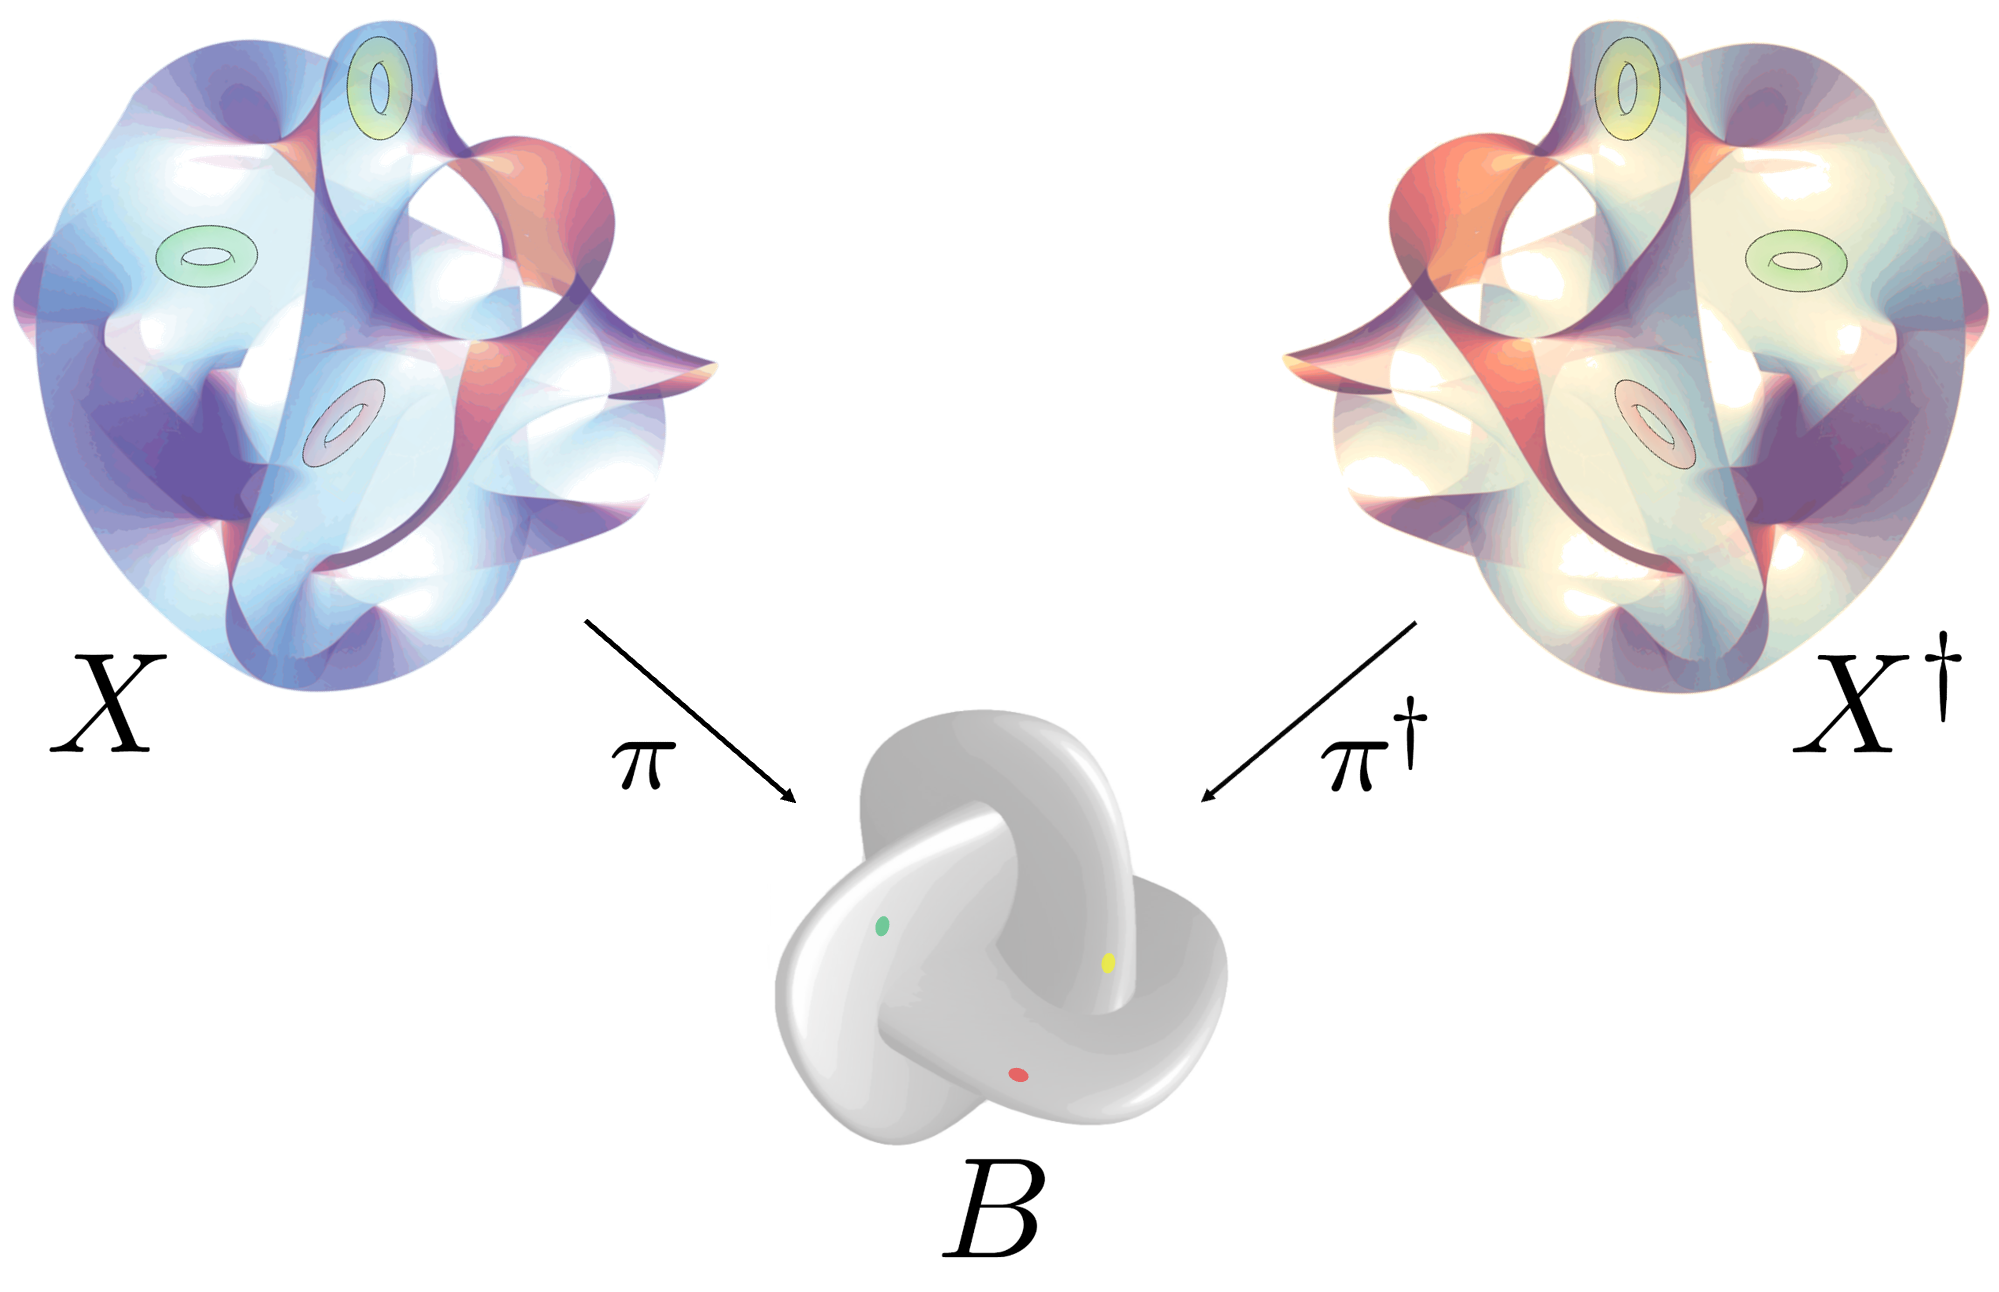
\includegraphics[width=0.62\linewidth]{fig15.png}
  \caption{SYZ 猜想把镜像 Calabi--Yau 流形对 $(X,X^\dagger)$ 的纤维（特殊拉格朗日环面）联系起来。（来源：\url{http://hci.stanford.edu/~cagatay/projects/boys/Demiralp-2009-CLF.pdf}、\url{https://plus.maths.org/content/hidden-dimensions}；特别感谢 KoMa，他建议了编辑此图及许多其他图的最佳方式。）\hfill（原书 p.127）}
  \label{fig:15}
\end{figure}
